\documentclass[preprint, 3p,
authoryear]{elsarticle} %review=doublespace preprint=single 5p=2 column
%%% Begin My package additions %%%%%%%%%%%%%%%%%%%

\usepackage[hyphens]{url}

  \journal{Transport Geography?} % Sets Journal name

\usepackage{graphicx}
%%%%%%%%%%%%%%%% end my additions to header

\usepackage[T1]{fontenc}
\usepackage{lmodern}
\usepackage{amssymb,amsmath}
% TODO: Currently lineno needs to be loaded after amsmath because of conflict
% https://github.com/latex-lineno/lineno/issues/5
\usepackage{lineno} % add
\usepackage{ifxetex,ifluatex}
\usepackage{fixltx2e} % provides \textsubscript
% use upquote if available, for straight quotes in verbatim environments
\IfFileExists{upquote.sty}{\usepackage{upquote}}{}
\ifnum 0\ifxetex 1\fi\ifluatex 1\fi=0 % if pdftex
  \usepackage[utf8]{inputenc}
\else % if luatex or xelatex
  \usepackage{fontspec}
  \ifxetex
    \usepackage{xltxtra,xunicode}
  \fi
  \defaultfontfeatures{Mapping=tex-text,Scale=MatchLowercase}
  \newcommand{\euro}{€}
\fi
% use microtype if available
\IfFileExists{microtype.sty}{\usepackage{microtype}}{}
\usepackage[]{natbib}
\bibliographystyle{plainnat}

\usepackage{graphicx}
\ifxetex
  \usepackage[setpagesize=false, % page size defined by xetex
              unicode=false, % unicode breaks when used with xetex
              xetex]{hyperref}
\else
  \usepackage[unicode=true]{hyperref}
\fi
\hypersetup{breaklinks=true,
            bookmarks=true,
            pdfauthor={},
            pdftitle={Social needs for transport and gaps in transit service: new GTFS tools},
            colorlinks=false,
            urlcolor=blue,
            linkcolor=magenta,
            pdfborder={0 0 0}}

\setcounter{secnumdepth}{5}
% Pandoc toggle for numbering sections (defaults to be off)


% tightlist command for lists without linebreak
\providecommand{\tightlist}{%
  \setlength{\itemsep}{0pt}\setlength{\parskip}{0pt}}




\usepackage{subfig}
\usepackage{booktabs}
\usepackage{longtable}
\usepackage{array}
\usepackage{multirow}
\usepackage{wrapfig}
\usepackage{float}
\usepackage{colortbl}
\usepackage{pdflscape}
\usepackage{tabu}
\usepackage{threeparttable}
\usepackage{threeparttablex}
\usepackage[normalem]{ulem}
\usepackage{makecell}
\usepackage{xcolor}



\begin{document}


\begin{frontmatter}

  \title{Social needs for transport and gaps in transit service: new
GTFS tools}
    \author[Public Transport Research Group (PTRG)]{James Reynolds%
  %
  \fnref{1}}
   \ead{james.reynolds@monash.edu} 
    \author[Public Transport Research Group (PTRG)]{Graham Currie%
  \corref{cor1}%
  \fnref{2}}
   \ead{graham.currie@monash.edu} 
    \author[Public Transport Research Group (PTRG)]{Yanda Qu%
  %
  \fnref{3}}
   \ead{yanda.qu@monash.edu} 
      \affiliation[Public Transport Research Group (PTRG)]{
    organization={Public Transport Research Group (PTRG), Institute of
Transport Studies, Department of Civil Engineering Engineering, Monash
University},addressline={Clayton
Campus},city={Melbourne},postcode={3800},state={Victoria},country={Australia},}
    \cortext[cor1]{Corresponding author}
    \fntext[1]{Research Fellow}
    \fntext[2]{Professor}
    \fntext[3]{PhD Student}
  
  \begin{abstract}
  This is the abstract.

  It consists of two paragraphs.
  \end{abstract}
    \begin{keyword}
    keyword1 \sep 
    keyword2
  \end{keyword}
  
 \end{frontmatter}

\section{Introduction}\label{introduction}

A common role for transit in many locations is to provide some mobility
for those who cannot otherwise drive themselves, so they can access
activities and services beyond walking distance \citep{Currie:2016aa}.
Age, disability, socio-economic status, lack of a vehicle or many other
reasons might make someone reliant on transit for some or all of their
travel. As well, fewer younger people are obtaining a driving license
than was the case previously \citep{delbosc2013causes}, suggesting that
there may be an increasing need for basic transit coverage in the
future.

Vertical social-equity perspectives on transport policy-making relate to
supporting those who are disadvantaged \citep{Litman:2016aa} and might
suggest providing at least some transit, and probably more than just a
minimum, where there are higher social needs for transport. Along these
lines \citet{Currie2003Hobart}, \citet{Currie2004Gap};
\citet{Currie2007Identifying} and \citet{currie2010identifying}
developed an approach for identifying spatial gaps in transit supply
related to social needs for transport, and applied it to a case study of
Melbourne in 2006.

However, there does not appear to have been much further use or
development of this spatial analysis technique. As well, it is unclear
whether the spatial patterns identified for Melbourne in 2006 have
changed in the intervening years, or if they are representative of other
places. This may in part be because, until recently, schedules were not
available in a consistent electronic format, meaning that assessing
transit supply was a large task requiring bespoke sourcing, cleaning and
analysis of data for each operator. Nowadays, however, more than 10,000
transit agencies publicly release timetable data in the General Transit
Feed Specification (GTFS) format \citep{GTFS}. Such standardisation
allows Google Maps and other online platforms to provide transit-related
outputs for any place publishing a feed, but tools for using GTFS data
to examine spatial patterns and gaps in transit supply with respect to
social needs for transport do not appear to be readily available. This
gap, and the lack of direct follow up to \citet{Currie2003Hobart},
\citet{Currie2004Gap}, \citet{Currie2007Identifying} and
\citet{currie2010identifying}, provide motivation for the research
reported in this paper.

The objectives of this research are: (1) to develop tools for
undertaking needs-gap analysis using GTFS datasets; and (2) to better
understand spatial patterns of gaps between social needs for transport
and transit supply, including whether those reported in
\citet{Currie2007Identifying} and \citet{currie2010identifying} are
representative of the current situation in Melbourne and elsewhere. This
paper reports the development of a new R package (gtfssupplyindex) with
tools for undertaking social needs-gaps analysis with GTFS datasets.
Also presented in this paper are results for Melbourne in 2016 and 2021,
matching the most recent censuses, for comparison to the 2006 results
reported in \citet{currie2010identifying}\footnote{The wider programme
  of research includes examination of spatial gaps in other cities, so
  as to better understand whether patterns in Melbourne are
  representative of other places. However, this paper is limited to
  examining Melbourne in 2016 and 2021 only. Results for other cities
  will be reported elsewhere.}.

The remainder of this paper is structured as follows: the next section
outlines the research context; Section 3 describes the study
methodology; results are presented in Section 4 and discussed in Section
5; and limitations of this study and directions for future research are
discussed in Section 6, which concludes the paper.

\section{Research context}\label{research-context}

There are many metrics available for assessing transit services.
Examples include: those in the \emph{Transit Cooperative Research
Program (TCRP) Report 88: a guidebook for developing
performance-measurement systems} \citep{Ryus:2003aa}; and those used
across benchmarking databases and programs such as by
\citet{Florida-Transit-Information-System:2018aa}, \citet{UITP:2015aa}
and \citet{Imperial-College-London:2023aa}. The Fielding Triangle
\citep{FieldingGordonJ1987Mpts} provides a framework for combining
indicators of service inputs, outputs and consumption to describe cost
efficiency, cost effectiveness and service effectiveness. More broadly:
\citet{Litman:2003ab} and \citet{Litman:2016aa} discuss the traffic,
mobility, accessibility, social equity, strategic planning and other
rational decision-making perspectives underlying many transport
indicators; \citet{Reynolds:2017ah} extends these into models of how
institutionalism, incrementalism and other public policy analysis
concepts might apply to transit prioritisation;
\citet{GuzmanLuisA.2017Aeit} developed a measure of accessibility in the
context of policy development and social equity for Latin American Bus
Rapid Transit (BRT) networks; and
\citet{Creutzig2020streetspaceallocation} introduced street space
allocation metrics based around ten ethical principles.

Many such metrics, however, may be difficult to calculate, understand or
use, especially for those who are not planners, engineers or other
technical specialists. Where pre-calculated transit metrics are
immediately available, it may not be possible to independently generate
scores or to assess proposed system changes. Contrasting examples are
provided by:

\begin{itemize}
\item
  \emph{Transit Score}s \citep{WalkScore:2023tg}, which are readily
  available online and provide a rating out of 100 (representing the
  sort of transit accessibility experienced in the center of New York),
  but which cannot be calculated independently.
\item
  The \emph{Transit Capacity and Quality of Service Manual (TCQSM)}
  \citep{TCQSM:2013}, which provides metrics for grouping many aspects
  of a transit system into five categories (very good to not very good)
  and which can be independently calculated (with sufficient data).
\end{itemize}

GTFS datasets have allowed the application of such metrics to many
transit systems. The \emph{Transit Score} website provides an example,
providing scores for places publishing a data feed. \citet{Wong:2013aa}
provides another in reporting the distribution of various \emph{TCQSM}
metrics across 50 USA transit operators. Code used in the
\citet{Wong:2013aa} analysis is available for those who might wish to
produce similar analysis for other locations or time periods. The lack
of a similar code base for calculating spatial gaps in transit supply
with respect to social needs for transport provides motivation for the
research reported in this paper.

\subsection{The Suppy Index (SI), Social Needs Index, and
Needs-gap}\label{the-suppy-index-si-social-needs-index-and-needs-gap}

The approach outlined in \citet{currie2010identifying} involved
calculating scores for geographical areas of interest across a Transit
Supply Index (SI) and a Composite Social Needs Index. These were then
used to identify areas with Very High needs, but Very Low or Zero
transit supply.

A generalized form of the Supply Index (SI) equation, adapted from
\citet{currie2010identifying}, is:

\[SI_{area, time} = \sum{\frac{Area_{Bn}}{Area_{area}}SL_{n, time}}\]

where:

\begin{itemize}
\item
  \(SI_{area, time}\) is the Supply Index for the area of interest and a
  given period of time;
\item
  \(Area_{Bn}\) is the buffer area for each stop (n) within the area of
  interest (in \citet{currie2010identifying} this was based on a radius
  of 400 metres for bus and tram stops, and 800 metres for railway
  stations);
\item
  \(Area_{area}\) is the area of the area of interest; and
\item
  \(SL_{n,time}\) is the number of transit arrivals for each stop for a
  given time period.
\end{itemize}

\begin{figure}

{\centering \subfloat[Distribution of Transit Supply\label{fig:Currie_map_SI-1}]{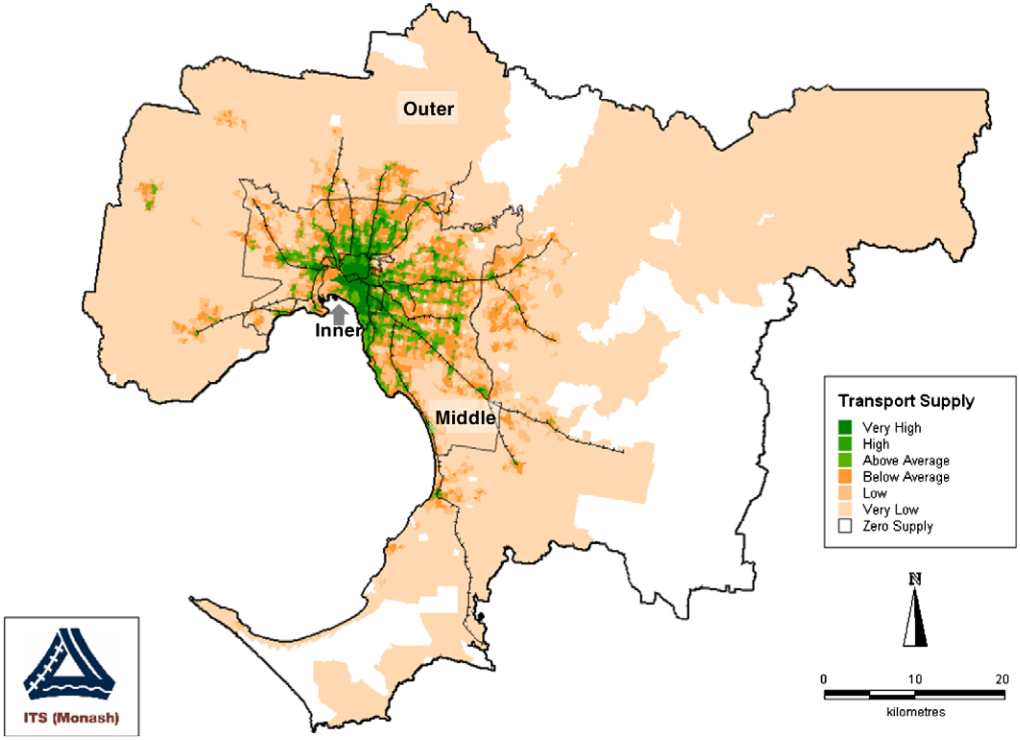
\includegraphics[width=0.5\linewidth]{graphics/Currie2010SI} }\subfloat[Distibution of Social Need for Transport\label{fig:Currie_map_SI-2}]{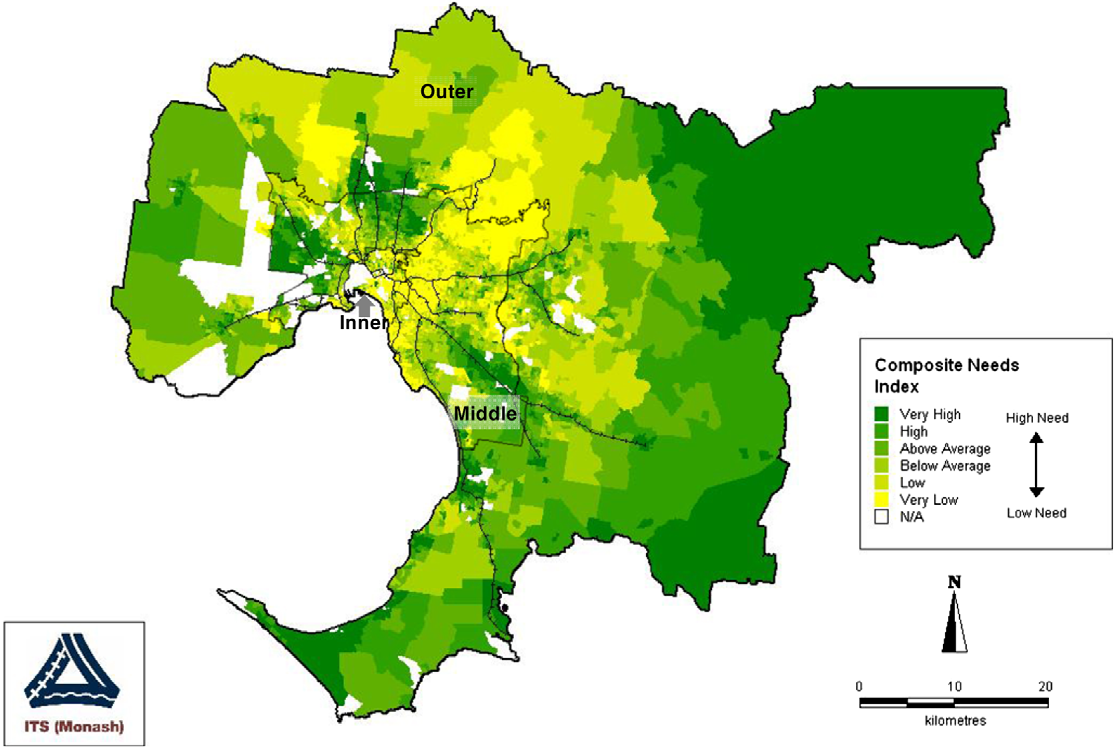
\includegraphics[width=0.5\linewidth]{graphics/Currie2010Needs} }\newline\subfloat[Supply Index and Composite Needs Index scores\label{fig:Currie_map_SI-3}]{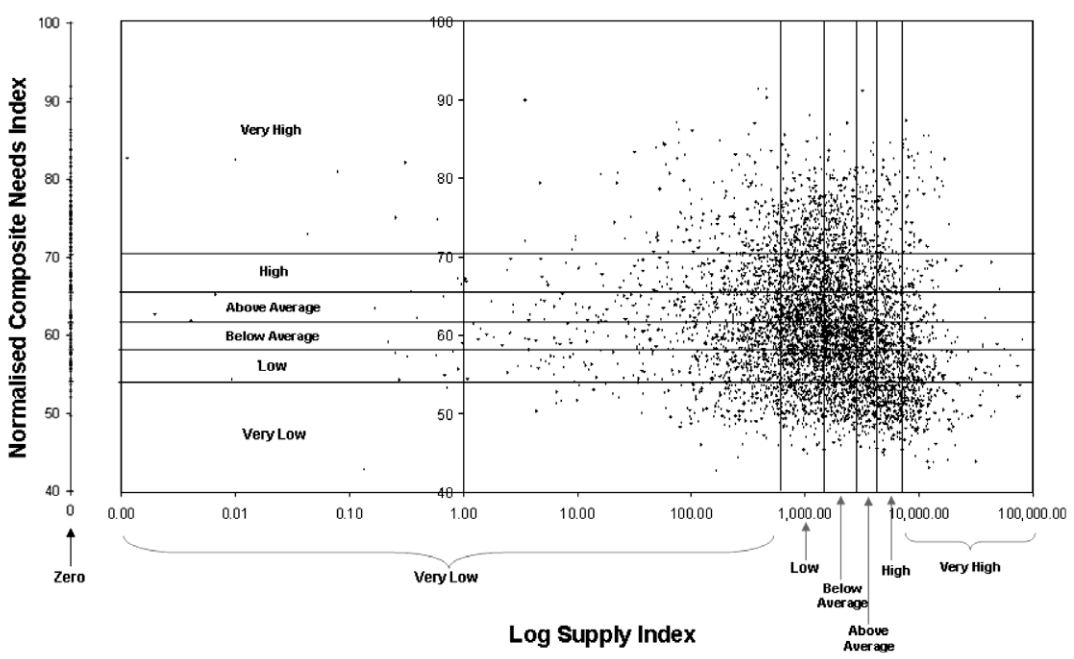
\includegraphics[width=0.5\linewidth]{graphics/Currie2010chart} }\subfloat[CCDs with Very High needs and Very Low or Zero supply\label{fig:Currie_map_SI-4}]{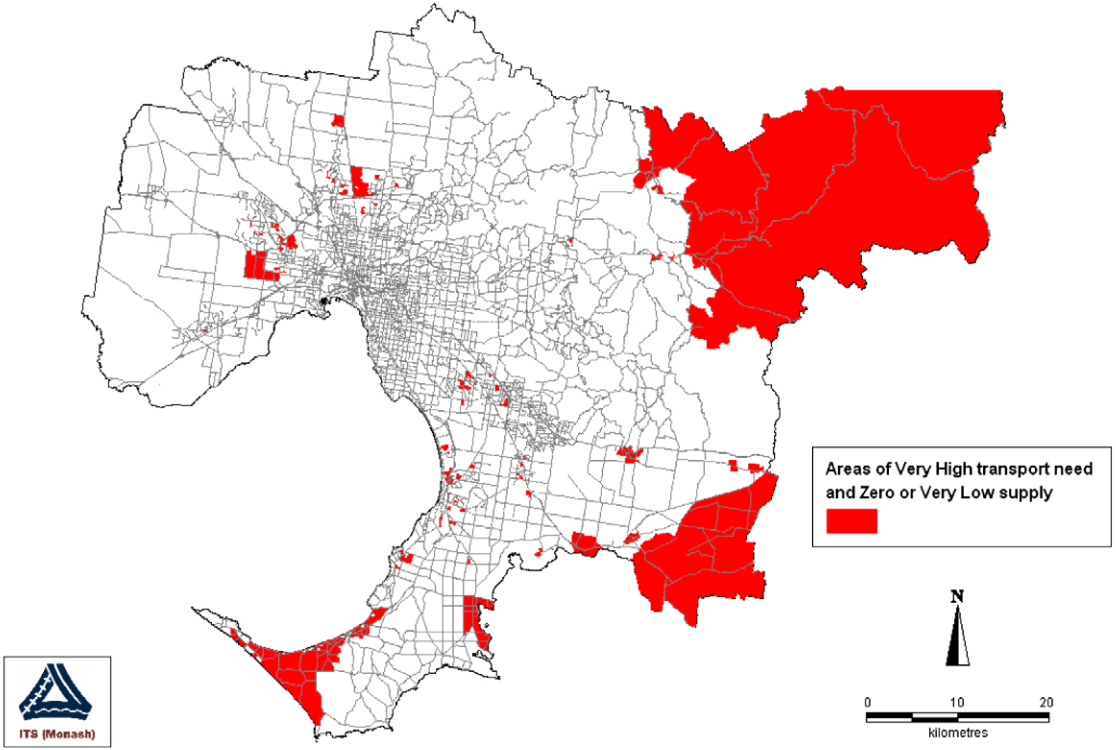
\includegraphics[width=0.5\linewidth]{graphics/Currie2010gap} }\newline

}

\caption{Melbourne 2006 Social Needs-Gap Results. Source: Currie (2010)}\label{fig:Currie_map_SI}
\end{figure}

\citet{currie2010identifying} reported SI scores for Census Collection
Districts (CCDs) across Melbourne in 2006. These were used to categorise
service levels into seven groups, as shown in Figure
\ref{fig:Currie_map_SI}(a). General patterns were identified, being:
more transit supply in the inner and middle suburbs, and along passenger
railway lines; and outer areas tending to have very low supply or no
transit at all.

\citet{currie2010identifying} assessed the social need for transport
across Melbourne using a composite index including: the Australian
Bureau of Statistics' (ABS') Index of Related Socio-Economic
Advantage/Disadvantage (IRSAD) and a transport needs index derived from
eight weighted indicators. The spatial distribution of this composite
social needs index, reproduced in Figure \ref{fig:Currie_map_SI}(b),
showed that areas of Above Average, High and Very High social needs were
located in: some outer suburbs, particularly in the east and south-east;
and in some middle suburbs in the south-east, north and west.

\citet{currie2010identifying} compared the Composite Social Needs Index
and Supply Index scores (Figure \ref{fig:Currie_map_SI}(c)) and
identified areas with Very High transport needs, but Very Low or Zero
transit supply (Figure \ref{fig:Currie_map_SI}(d)), where service gaps
might be of particular concern. Most of these were located in the outer
suburbs of Melbourne in the north-east, south-east and south, although
there were also some pockets in the middle suburbs in the west, north
and south east. Overall, ``8.2\% of Melbourne residents ha(d) `very
high' needs but `zero', `low' or `very low' public transport
supply''\citep{currie2010identifying}.

This approach does not appear to have been adopted widely in practice or
by researchers. Our suspicion is that while the SI has a relatively
simple formula and requires only geographic and timetable data to
calculate, a lack of software tools to complete the analysis may be
partly why it has not been more widely adopted. The case-based methods
used in this research to develop such tools are discussed in the
following.

\section{Methodology}\label{methodology}

Case approaches can be particularly useful when research questions are
about `how' or `why', but researchers lack control of events (preventing
experiments)\citep{Yin2009aa}. Here the research questions relate to:
(1) how to use GTFS data to assess gaps between social needs and transit
supply, and (2) how and why spatial patterns might have changed since
those reported for 2006 in \citet{currie2010identifying}. There is no
ability here to control events so a case research approach appears well
suited to this study.

When using a case research approach there is also a need to address the
``duality criterion'', being seeking generalisable findings while at the
same time being grounded in the context of only a small number of cases
(allowing greater depth)\citep{Denscombe2007aa, Ketokivi2014aa}. Here
the approach taken has been to develop a package of tools for
calculating the SI from GTFS data using the R programming language
\citep{R-base}, so that the duality criterion is addressed by developing
generic software functions that might be applied to other GTFS feeds,
beyond the Melbourne case reported in this paper. The recommendations of
\citet{wickham2023r} informed the package setup and development
approach. Various existing packages and code examples were relied upon
including: the sf package \citep{R-sf} for geospatial analysis; the
tidyverse \citep{tidyverse2019}; gtfstools \citep{R-gtfstools}; and
tidytransit \citep{R-tidytransit}.

There are, however, limitations to the generalisability of this research
with respect to changes since 2006 and the patterns reported in
\citet{currie2010identifying}(research question 2).
\citet{Currie2007Identifying} and \citet{currie2010identifying} reported
results for Melbourne only, and while \citet{Currie2003Hobart} and
\citet{Currie2004Gap} reported results for Hobart and Adelaide, these
used earlier versions of the needs-gap assessment methodology, for which
software tools have not been developed here. While this study does seek
findings about changes in spatial patterns of social needs and transit
supply that are generalisable to more than just Melbourne, a lack of
2006 results for other cities may limit the extent to which these
findings might be confidently considered representative of changes in
other places\footnote{Other parts of this research programme will
  examine changes over the last 10-15 years in other cities (where GTFS
  data is available). The focus of this paper, however, is on Melbourne.}.

\subsection{Code developement}\label{code-developement}

Code was developed and tested on the Mornington Peninsula Tourist
Railway GTFS feed. This was selected primarily for convenience, given
that the authors are familiar with the surrounding geography and that
the feed covers only a small number of trips across just three stations
(thereby facilitating hand verification of outputs). ABS data was used
to define areas of interest, and was sourced via the absmapsdata package
\citep{R-absmapsdata}.

\subsection{Melbourne Case Study}\label{melbourne-case-study}

The methodological literature provides guidance on case selection and
discusses various theoretical sampling approaches, including sampling
for critical, particularly revelatory and/or representative cases
\citep{Eisenhardt1989aa, Yin2009aa, Denscombe2007aa, Eisenhardt2007TBfC}.
\citet{Yin2009aa} notes selection of a case to allow longitudinal study,
and this is the primary reason for selecting Melbourne here, so as to
facilitate comparison with the 2006 results reported in
\citet{currie2010identifying}. As such, SI scores were calculated using
the same Census Collection Districts (CCDs) used by
\citet{currie2010identifying}, but for the weeks starting the day of the
2016 and 2021 censuses. The Victorian GTFS feed, published by Public
Transport Victoria (PTV), was used, with historical feeds sourced from
\citet{transitfeeds_victoria:2023aa}.

Unfortunately, it is not possible to obtain 2016 or 2021 social
disadvantage data for CCDs, as the ABS no longer releases data using
this geographic scheme. Instead, population and other statistics are now
released for Statistical Area (SA) zones, under a hierarchical structure
ranging from SA1s (\textasciitilde400 people) to SA4s (parts of a city
or region)\citep{ABSmaps}. As such, SI scores have also been calculated
for SA1s, to facilitate use of ABS data to identify needs-gaps.

The same Transport Supply categorizations have been used as in
\citet{currie2010identifying}\footnote{Zero, Very Low, Low, Below
  average, Above average, High and Very High.}. As well, this study
adopts a similar approach to measuring social disadvantage as used in
\citet{currie2010identifying}, using: the ABS' IRSAD and a transport
needs index calculated from various other statistics \footnote{The same
  need indicators and weightings used in \citet{currie2010identifying}
  were adopted, although \$799 or lower per week was used as the
  threshold for low income households rather than \$499 to account for
  inflation (as per the Reserve Bank of Australia's online inflation
  calculator).}. A composite needs indicator was derived based on the
IRSAD and the transport needs index, again as per the
\citet{currie2010identifying} approach. However, changes to ABS
reporting means that the composite needs indicator used by
\citet{currie2010identifying} cannot be exactly replicated\footnote{The
  approach used here includes only two components in the composite needs
  index In contrast to the four of \citet{currie2010identifying}, which
  included two ``relative need'' components obtained by weighting the
  IRSAD and the transport needs indexes by the population within the
  various needs groups for each area of interest. Current ABS reporting,
  however, does not allow the total number of people within one or more
  of the various needs groups to be identified at the SA1 level.} based
on weighting both the IRSAD index and the transport need index by the
total population of each SA1. These were then standardised and grouped,
as per the six groups used by \citet{currie2010identifying}\footnote{Very
  Low, Low, Below average, Above average, High and Very High.}.

\section{Results}\label{results}

\subsection{The gtfssupplyindex
package}\label{the-gtfssupplyindex-package}

Code developed to calculate SI scores is available as an R package on
github (see \citet{gtfssupplyindex_github}). Included in the package is
a vignette (included as an Appendix to this paper) that outlines the
developed functions and provides step-by-step calculations for the
Mornington Peninsula Railway as a worked example.

\subsection{Melbourne}\label{melbourne}

\subsubsection{Transport Supply
Categories}\label{transport-supply-categories}

\begin{table}

\caption{\label{tab:Greater_Melbourne_CCDs_SA1_table}Distribution of 2006, 2016 and 2021 Transport Supply to Melbourne CCDs (2006 boundaries), 2016 Transport Supply to Greater Melbourne (2016 SA1s) and 2021 Transport Supply to Greater Melbourne (2021 SA1s). Sources: 2006 values, Currie (2010); 2016 and 2021 values, authors' analysis}
\centering
\begin{tabular}[t]{l|r|r|r|r|r}
\hline
\multicolumn{1}{c|}{Transport} & \multicolumn{3}{c|}{CCDs} & \multicolumn{1}{c|}{2016 SA1s} & \multicolumn{1}{c}{2021 SA1s} \\
\cline{1-1} \cline{2-4} \cline{5-5} \cline{6-6}
Supply & 2006 & 2016 & 2021 & 2016 & 2021\\
\hline
Zero Supply & 3.2\%   (189) & 1.4\%    (86) & 1.3\%    (81) & 3.2\%    (326) & 4.3\%    (489)\\
\hline
Very Low & 22.5\% (1,314) & 23.5\% (1,485) & 23.3\% (1,474) & 23.0\%  (2,362) & 23.4\%  (2,692)\\
\hline
Low & 22.4\% (1,310) & 23.5\% (1,484) & 23.3\% (1,473) & 23.0\%  (2,362) & 23.4\%  (2,691)\\
\hline
Below average & 22.2\% (1,294) & 23.5\% (1,484) & 23.3\% (1,473) & 23.0\%  (2,362) & 23.4\%  (2,691)\\
\hline
Above average & 10.4\%   (608) & 9.4\%   (596) & 9.6\%   (608) & 9.3\%    (959) & 8.5\%    (975)\\
\hline
High & 9.2\%   (535) & 9.4\%   (595) & 9.6\%   (608) & 9.3\%    (959) & 8.5\%    (974)\\
\hline
Very High & 10.1\%   (589) & 9.4\%   (595) & 9.6\%   (608) & 9.3\%    (959) & 8.5\%    (975)\\
\hline
Total & 100.0\% (5,839) & 100.0\% (6,325) & 100.0\% (6,325) & 100.0\% (10,289) & 100.0\% (11,487)\\
\hline
\end{tabular}
\end{table}

Table \ref{tab:Greater_Melbourne_CCDs_SA1_table} summarises the
distribution of CCDs and SA1s across different Transport Supply
categories in 2006, 2016 and 2021. There is a statistically significant
difference in the shares of CCDs in each category between 2006, 2016 and
2021 (\(\chi^2(12, N = 18489) = 87.45\), \(p < .001\))\footnote{Differences
  are also statistically significant when comparing 2006 and 2016
  (\(\chi^2(6, N = 12164) = 56.87\), \(p < .001\)) or 2006 and 2021
  \(\chi^2(6, N = 12164) = 59.15\), \(p < .001\)), but not between 2016
  and 2021 (\(\chi^2(6, N = 12650) = 0.67\), \(p = .995\)).}. Only 81
CCDs (1.3\%) have Zero Supply in 2021, compared to the 189 (3.2\%)
reported by \citet{currie2010identifying} for 2006.

These shares by CCDs, however, are only for 2006 extents of Melbourne.
The ABS' statistical boundary of ``Greater Melbourne'' now includes
areas up to around 30 kilometers further to the north. Figure
\ref{fig:Greater_Melbourne_population_2021_by_SA4} shows the spatial
distribution of Transport Supply by SA1 in 2021, including all of the
SA1s within the 2021 Greater Melbourne Greater Capital City Statistical
Area (GCCSA). Additional maps showing Transport Supply by CCD and for
2016 are included in the Appendix. Figure
\ref{fig:Greater_Melbourne_population_2021_by_SA4} includes the 2006
boundary as an overlay, and\\
indicates that much of the new parts of Greater Melbourne have Very Low
or Zero Supply levels. In general, however, the spatial distribution of
Transport Supply is similar to that shown for 2006 in Figure
\ref{fig:Currie_map_SI}(a), with higher levels of Transport Supply in
more central areas and closer to suburban railway lines.

The difference between the share of areas of interest in each category
in 2006 (CCDs), 2016 and 2021 (SA1s) is also statistically significant
(\(\chi^2(12, N = 27615) = 58.86\), \(p < .001\))\footnote{Differences
  between 2006 and 2016, as a pair, are not statistically significant
  (\(\chi^2(6, N = 16128) = 8.83\), \(p = .183\)). Differences between
  2006 and 2021 are signficant (\(\chi^2(6, N = 17326) = 44.83\),
  \(p < .001\)) as are the differences between 2016 and 2021
  \(\chi^2(6, N = 21776) = 31.56\), \(p < .001\)).}. There is a greater
proportion of SA1s with Zero Supply in 2021 (4.3\%) than there were CCDs
in 2006 (3.25\%) or SA1s in 2016 (3.2\%). The share of SA1s with supply
below the average (i.e.~Zero, Very Low, Low or Below Average) is also
larger in 2021 (74.5\%) than the share of CCDs in 2006 (70.3\%) or share
of SA1s in 2016 (72.0\%).

\begin{table}

\caption{\label{tab:Greater_Melbourne_CCDs_SA1_population}Distribution of 2006, 2016 and 2021 Transport Supply to population in Melbourne. Sources: 2006 values, Currie (2010); 2016 and 2021 values, authors' analysis}
\centering
\begin{tabular}[t]{l|r|r|r}
\hline
Supply & 2006 & 2016 & 2021\\
\hline
Zero Supply & 2.5\%    (85,423) & 2.9\%   (131,619) & 3.8\%   (186,829)\\
\hline
Very Low & 23.6\%   (793,046) & 22.5\% (1,008,498) & 23.0\% (1,132,967)\\
\hline
Low & 25.7\%   (865,330) & 22.7\% (1,016,848) & 23.7\% (1,163,358)\\
\hline
Below average & 23.0\%   (774,521) & 22.3\% (1,000,290) & 23.6\% (1,159,783)\\
\hline
Above average & 9.6\%   (324,546) & 9.3\%   (418,614) & 8.7\%   (426,892)\\
\hline
High & 7.7\%   (260,411) & 9.6\%   (428,880) & 8.7\%   (425,779)\\
\hline
Very High & 7.8\%   (263,832) & 10.7\%   (480,469) & 8.6\%   (422,025)\\
\hline
Total & 100.0\% (3,367,109) & 100.0\% (4,485,218) & 100.0\% (4,917,633)\\
\hline
\end{tabular}
\end{table}

Table \ref{tab:Greater_Melbourne_CCDs_SA1_population} compares the share
of resident population in each transport supply category. Greater
Melbourne's population increased by 46\% between 2006 (3,367,109) and
2021 (3,367,109). However, the number of residents living in areas with
Zero Supply rose by 119\% from 85,423 (2.5\% of the total population) in
2006 to 186,829 (3.8\%) in 2021. Residents with Zero or Very Low
Transport Supply rose by 50\% from 878,469 (26.1\%) in 2006 to 1,319,796
(26.8\%) in 2021, while those with supply below the average (i.e.~Zero,
Very Low, Low or Below Average) rose by 45\% from 2,518,320 (74.8\%) in
2006 to 3,642,937 (74.1\%) in 2021. Between 2016 and 2021, Greater
Melbourne's population increased by 10\%, but the number of residents in
SA1s with Zero Supply rose by 42\%. The number of residents with Zero or
Very Low Transport Supply rose by 16\%, while residents with supply
below the average (Zero, Very Low, Low or Below Average) rose 15\%.

\begin{table}

\caption{\label{tab:Greater_Melbourne_population_2016_by_SA4}Greater Melbourne 2016: Share of population in each Transport Supply category for each SA4 region}
\centering
\fontsize{8}{10}\selectfont
\begin{tabular}[t]{>{\raggedright\arraybackslash}p{1.75cm}|>{\raggedleft\arraybackslash}p{1cm}|>{\raggedleft\arraybackslash}p{1cm}|>{\raggedleft\arraybackslash}p{1cm}|>{\raggedleft\arraybackslash}p{1cm}|>{\raggedleft\arraybackslash}p{1cm}|>{\raggedleft\arraybackslash}p{1cm}|>{\raggedleft\arraybackslash}p{1cm}|>{\raggedright\arraybackslash}p{1cm}|>{\raggedleft\arraybackslash}p{1cm}|>{\raggedleft\arraybackslash}p{1.25cm}}
\hline
Transport Supply & Inner & Inner East & Inner South & North East & North West & Outer East & South East & West & M'ton Pen. & Total\\
\hline
Zero Supply & 0.0\%       (0) & 0.0\%     (480) & 0.0\%   (1,604) & 0.4\%  (16,988) & 0.4\%  (17,655) & 0.3\%  (12,955) & 1.0\%  (44,757) & 0.3\%  (12,056) & 0.6\%  (25,124) & 2.9\%   (131,619)\\
\hline
Very Low & 0.1\%   (3,427) & 0.4\%  (18,454) & 0.6\%  (24,944) & 2.5\% (112,269) & 2.1\%  (94,853) & 4.3\% (190,890) & 4.8\% (215,217) & 4.2\% (186,665) & 3.6\% (161,779) & 22.5\% (1,008,498)\\
\hline
Low & 0.4\%  (18,018) & 0.9\%  (39,235) & 1.4\%  (60,833) & 2.7\% (119,608) & 2.4\% (107,693) & 3.0\% (135,247) & 5.0\% (224,097) & 5.4\% (242,438) & 1.6\%  (69,679) & 22.7\% (1,016,848)\\
\hline
Below average & 1.0\%  (42,950) & 2.3\% (105,168) & 2.9\% (128,014) & 2.9\% (132,008) & 2.2\%  (97,739) & 2.7\% (119,691) & 4.0\% (177,817) & 3.8\% (170,015) & 0.6\%  (26,888) & 22.3\% (1,000,290)\\
\hline
Above average & 1.0\%  (44,547) & 1.8\%  (80,002) & 1.8\%  (81,038) & 1.0\%  (46,965) & 0.6\%  (28,905) & 0.6\%  (25,188) & 1.2\%  (53,228) & 1.2\%  (54,895) & 0.1\%   (3,846) & 9.3\%   (418,614)\\
\hline
High & 2.9\% (129,533) & 1.7\%  (74,966) & 1.7\%  (74,617) & 1.0\%  (46,291) & 0.3\%  (14,464) & 0.3\%  (15,371) & 0.7\%  (33,365) & 0.9\%  (38,499) & 0.0\%   (1,774) & 9.6\%   (428,880)\\
\hline
Very High & 7.9\% (353,232) & 0.9\%  (41,416) & 0.7\%  (32,561) & 0.5\%  (21,197) & 0.0\%   (2,033) & 0.0\%     (314) & 0.2\%   (6,893) & 0.5\%  (22,823) & 0.0\%       (0) & 10.7\%   (480,469)\\
\hline
Total & 13.2\% (591,707) & 8.0\% (359,721) & 9.0\% (403,611) & 11.0\% (495,326) & 8.1\% (363,342) & 11.1\% (499,656) & 16.8\% (755,374) & 16.2\% (727,391) & 6.4\% (289,090) & 100.0\% (4,485,218)\\
\hline
\end{tabular}
\end{table}

\begin{table}

\caption{\label{tab:Greater_Melbourne_population_2021_by_SA4}Greater Melbourne 2021: Share of population in each Transport Supply category for each SA4 region}
\centering
\fontsize{8}{10}\selectfont
\begin{tabular}[t]{>{\raggedright\arraybackslash}p{1.75cm}|>{\raggedleft\arraybackslash}p{1cm}|>{\raggedleft\arraybackslash}p{1cm}|>{\raggedleft\arraybackslash}p{1cm}|>{\raggedleft\arraybackslash}p{1cm}|>{\raggedleft\arraybackslash}p{1cm}|>{\raggedleft\arraybackslash}p{1cm}|>{\raggedleft\arraybackslash}p{1cm}|>{\raggedright\arraybackslash}p{1cm}|>{\raggedleft\arraybackslash}p{1cm}|>{\raggedleft\arraybackslash}p{1.25cm}}
\hline
Transport Supply & Inner & Inner East & Inner South & North East & North West & Outer East & South East & West & M'ton Pen. & Total\\
\hline
Zero Supply & 0.0\%       (0) & 0.0\%     (478) & 0.0\%   (1,655) & 0.5\%  (26,563) & 0.5\%  (22,186) & 0.3\%  (14,125) & 1.1\%  (53,966) & 0.9\%  (43,898) & 0.5\%  (23,958) & 3.8\%   (186,829)\\
\hline
Very Low & 0.1\%   (4,169) & 0.4\%  (20,688) & 0.5\%  (22,483) & 2.7\% (130,715) & 2.3\% (110,814) & 4.1\% (200,810) & 5.1\% (250,684) & 4.5\% (221,337) & 3.5\% (171,267) & 23.0\% (1,132,967)\\
\hline
Low & 0.4\%  (20,329) & 0.9\%  (45,160) & 1.3\%  (63,802) & 2.7\% (132,001) & 2.5\% (123,314) & 3.2\% (155,603) & 5.4\% (265,995) & 5.9\% (289,518) & 1.4\%  (67,636) & 23.7\% (1,163,358)\\
\hline
Below average & 1.1\%  (54,918) & 2.7\% (133,305) & 3.0\% (148,585) & 3.1\% (151,240) & 2.6\% (129,918) & 2.3\% (114,658) & 4.2\% (204,093) & 3.8\% (184,466) & 0.8\%  (38,600) & 23.6\% (1,159,783)\\
\hline
Above average & 1.1\%  (56,422) & 1.4\%  (69,199) & 1.9\%  (92,875) & 0.9\%  (44,470) & 0.6\%  (27,140) & 0.5\%  (22,262) & 1.1\%  (53,328) & 1.1\%  (55,438) & 0.1\%   (5,758) & 8.7\%   (426,892)\\
\hline
High & 3.1\% (151,439) & 1.5\%  (73,687) & 1.4\%  (69,281) & 0.9\%  (43,985) & 0.2\%   (9,710) & 0.2\%  (10,905) & 0.5\%  (24,707) & 0.8\%  (41,100) & 0.0\%     (965) & 8.7\%   (425,779)\\
\hline
Very High & 6.7\% (329,654) & 0.6\%  (30,949) & 0.5\%  (23,906) & 0.2\%  (11,752) & 0.0\%   (1,285) & 0.0\%       (0) & 0.1\%   (7,308) & 0.3\%  (17,171) & 0.0\%       (0) & 8.6\%   (422,025)\\
\hline
Total & 12.5\% (616,931) & 7.6\% (373,466) & 8.6\% (422,587) & 11.0\% (540,726) & 8.6\% (424,367) & 10.5\% (518,363) & 17.5\% (860,081) & 17.3\% (852,928) & 6.3\% (308,184) & 100.0\% (4,917,633)\\
\hline
\end{tabular}
\end{table}

\begin{figure}
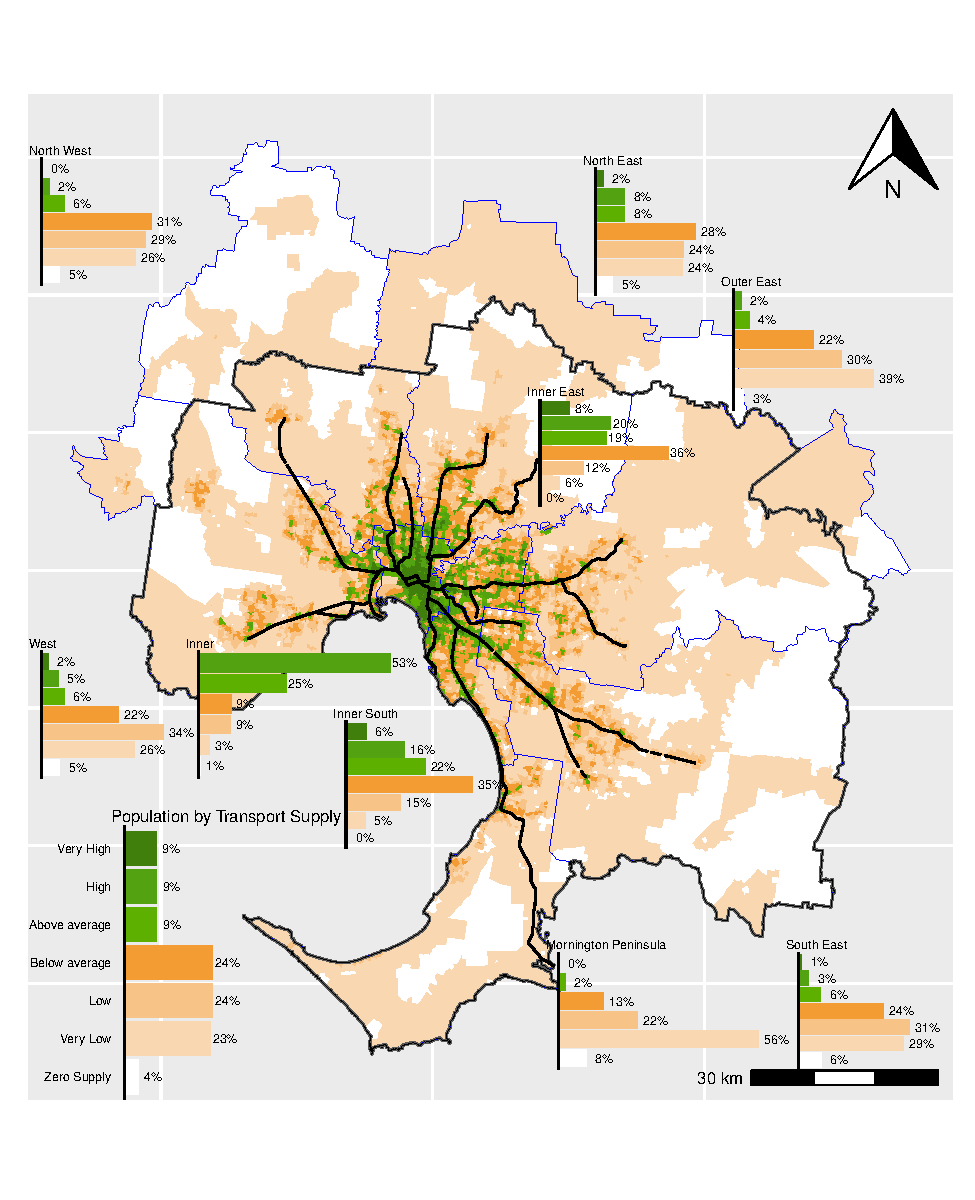
\includegraphics[width=1\linewidth]{ReynoldsCurrieQu2024_files/figure-latex/Greater_Melbourne_population_2021_by_SA4-1} \caption{Greater Melbourne 2021: Transport Supply by SA1,  overlayed with suburban rail network (black), SA4 boundaries (blue) and 2006 Melbourne extents (black)}\label{fig:Greater_Melbourne_population_2021_by_SA4}
\end{figure}

Variations in the share of SA1s in each Transport Supply category across
SA4 zones are statistically significant in both 2016
(\(\chi^2(48, N = 10289) = 6195.85\), \(p < .001\)) and 2021
(\(\chi^2(48, N = 11487) = 7250.39\), \(p < .001\))\footnote{Tables
  showing Transport Supply by number of SA1s for each SA4 are included
  in the Appendix.}. Tables
\ref{tab:Greater_Melbourne_population_2016_by_SA4} and
\ref{tab:Greater_Melbourne_population_2021_by_SA4} show the population
in each supply category by SA4 for 2016 and 2021. In general, larger
shares of residents have lower than the average supply in outer areas of
Greater Melbourne\footnote{The North East, North West, Outer East, South
  East, West and Mornington Peninsula SA4 zones}. In 2016, 2,714,128
residents (60.5\% of the total population of Greater Melbourne) were
both living outside of the inner three SA4s and in SA1s with lower than
average supply. By 2021 this had increased to 3,127,365 residents
(63.6\%).

\subsubsection{Supply Index scores}\label{supply-index-scores}

\citet{currie2010identifying} reported an average SI score for CCDs in
2006 of 2,886.9 across Melbourne, with averages of 10,922.7, 2,694.9 and
764.3 across the inner, middle and outer suburbs, respectively. In
comparison, the average SI value found here for 2021 (using CCDs and
within the 2006 boundary) is 3,390, 12,275.7 (+12\%), 3,409.1 (+27\%)
and 998.96 (+31\%) for the inner, middle and outer suburbs
respectively\footnote{The same grouping of Local Government Areas (LGAs)
  to inner, middle and outer suburb groups as used in
  \citet{currie2010identifying} was used for this analysis, although
  here the City of Stonnington was allocated entirely to the middle
  grouping, whereas \citet{currie2010identifying} allocated part of this
  LGA to the inner group.}. However, average scores found here might not
be exactly comparable to those in \citet{currie2010identifying} due to
geographic inconsistencies\footnote{The \citet{currie2010identifying}
  results show 5,839 total CCDs within Melbourne, whereas the shape
  files obtained for this analysis include 6,325 CCDs within the 2006
  Melbourne boundary.}. Overall, however, the results appear to be
consistent with there having been increases in SI scores across all
parts of Melbourne since 2006, while the general pattern of higher
average SI scores in inner (and then middle) suburbs than in outer
suburbs remains unchanged.

\begin{table}

\caption{\label{tab:Greater_Melbourne_2016_2021_ratio_map}Greater Melbourne: Share of 2021 population living in SA1s by change in transit service (2016 vs 2021) by SA4 region}
\centering
\fontsize{8}{10}\selectfont
\begin{tabular}[t]{>{\raggedright\arraybackslash}p{1.75cm}|>{\raggedleft\arraybackslash}p{1cm}|>{\raggedleft\arraybackslash}p{1cm}|>{\raggedleft\arraybackslash}p{1cm}|>{\raggedleft\arraybackslash}p{1cm}|>{\raggedleft\arraybackslash}p{1cm}|>{\raggedleft\arraybackslash}p{1cm}|>{\raggedleft\arraybackslash}p{1cm}|>{\raggedright\arraybackslash}p{1cm}|>{\raggedleft\arraybackslash}p{1cm}|>{\raggedleft\arraybackslash}p{1.25cm}}
\hline
Change & Inner & Inner East & Inner South & North East & North West & Outer East & South East & West & M'ton Pen. & Total\\
\hline
New service & 0.0\%       (0) & 0.0\%       (0) & 0.0\%       (0) & 0.2\%   (9,911) & 0.7\%  (36,817) & 0.0\%     (238) & 1.1\%  (53,254) & 0.8\%  (40,483) & 0.1\%   (3,038) & 2.9\%   (143,741)\\
\hline
Increased 30\% or more & 0.0\%   (1,843) & 0.0\%     (279) & 0.8\%  (37,932) & 0.9\%  (46,448) & 1.7\%  (83,007) & 0.1\%   (4,209) & 2.6\% (127,248) & 2.7\% (131,194) & 1.3\%  (65,724) & 10.1\%   (497,884)\\
\hline
Increased 10 to 30\% & 0.9\%  (45,197) & 0.1\%   (3,190) & 0.8\%  (41,577) & 0.8\%  (40,989) & 1.1\%  (56,013) & 0.5\%  (22,609) & 1.6\%  (77,391) & 2.1\% (101,767) & 0.4\%  (21,060) & 8.3\%   (409,793)\\
\hline
Increased 5 to 10\% & 1.5\%  (72,360) & 0.3\%  (13,018) & 1.1\%  (52,033) & 0.8\%  (37,258) & 0.6\%  (31,400) & 0.5\%  (26,666) & 1.1\%  (53,370) & 2.1\% (101,769) & 0.2\%  (10,149) & 8.1\%   (398,023)\\
\hline
Increased 3 to 5\% & 1.6\%  (79,047) & 0.5\%  (25,074) & 0.6\%  (30,595) & 1.2\%  (60,661) & 1.1\%  (55,445) & 0.5\%  (23,819) & 0.9\%  (45,773) & 1.8\%  (88,601) & 0.3\%  (14,666) & 8.6\%   (423,681)\\
\hline
Increased 1 to 3\% & 2.3\% (115,203) & 1.4\%  (67,357) & 1.2\%  (60,889) & 1.9\%  (92,896) & 0.9\%  (42,761) & 0.8\%  (39,263) & 1.5\%  (75,676) & 2.4\% (117,967) & 0.7\%  (32,811) & 13.1\%   (644,823)\\
\hline
Within 1\% & 2.6\% (128,666) & 3.8\% (187,974) & 2.0\%  (97,037) & 2.5\% (124,942) & 1.2\%  (57,899) & 5.6\% (274,423) & 5.4\% (266,787) & 3.0\% (146,702) & 2.2\% (109,151) & 28.3\% (1,393,581)\\
\hline
Reduced 1 to 3\% & 1.0\%  (49,729) & 0.8\%  (39,675) & 0.6\%  (27,179) & 0.7\%  (34,180) & 0.3\%  (13,986) & 0.8\%  (38,826) & 0.7\%  (34,125) & 0.4\%  (19,517) & 0.4\%  (18,446) & 5.6\%   (275,663)\\
\hline
Reduced 3 to 10\% & 1.8\%  (89,662) & 0.5\%  (25,930) & 0.9\%  (42,701) & 0.9\%  (44,261) & 0.2\%  (11,175) & 0.9\%  (43,143) & 0.5\%  (24,903) & 0.7\%  (33,329) & 0.2\%   (7,953) & 6.6\%   (323,057)\\
\hline
Reduced 10\% or more & 0.7\%  (35,224) & 0.2\%  (10,491) & 0.6\%  (30,989) & 0.5\%  (22,617) & 0.3\%  (13,678) & 0.6\%  (31,042) & 1.0\%  (47,588) & 0.6\%  (27,701) & 0.0\%   (1,228) & 4.5\%   (220,558)\\
\hline
Service withdrawn (magenta) & 0.0\%       (0) & 0.0\%       (0) & 0.0\%       (0) & 0.0\%   (1,777) & 0.0\%     (424) & 0.0\%   (1,270) & 0.0\%   (1,360) & 0.0\%   (1,015) & 0.0\%       (0) & 0.1\%     (5,846)\\
\hline
Never served (black) & 0.0\%       (0) & 0.0\%     (478) & 0.0\%   (1,655) & 0.5\%  (24,786) & 0.4\%  (21,762) & 0.3\%  (12,855) & 1.1\%  (52,606) & 0.9\%  (42,883) & 0.5\%  (23,958) & 3.7\%   (180,983)\\
\hline
Total & 12.5\% (616,931) & 7.6\% (373,466) & 8.6\% (422,587) & 11.0\% (540,726) & 8.6\% (424,367) & 10.5\% (518,363) & 17.5\% (860,081) & 17.3\% (852,928) & 6.3\% (308,184) & 100.0\% (4,917,633)\\
\hline
\end{tabular}
\end{table}

\begin{figure}
\centering
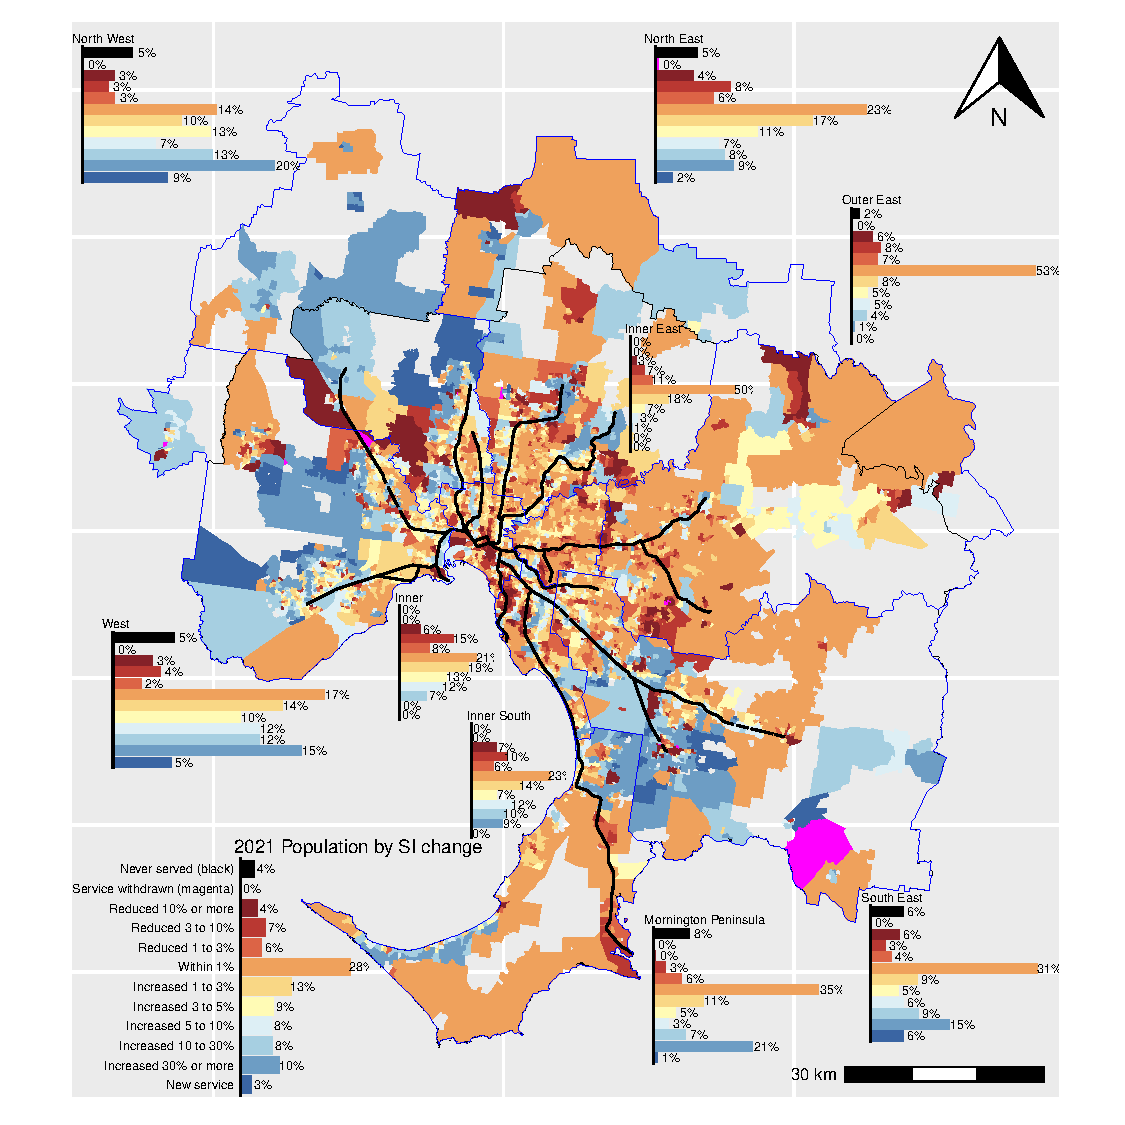
\includegraphics{ReynoldsCurrieQu2024_files/figure-latex/Greater_Melbourne_2016_2021_ratio_map-1.pdf}
\caption{Greater Melbourne: changes in SI between 2016 and 2021, by 2021
SA1, overlayed with 2006 Greater Melbourne boundary (black); 2021 SA4
boundaries (blue); and suburban railway lines (black)}
\end{figure}

Average SI scores for SA1s across all of Greater Melbourne increased
from 2,843.8 in 2016 to 2,901.4 in 2021, (+2.0\%). There is a
statistically significant correlation between the 2016 and 2021 SI
scores (\(r(11485) = 1.00\), \(p < .001\), \(r_s =.98\), \(p < .001\)).
Figure \ref{fig:Greater_Melbourne_2016_2021_ratio_map} shows changes in
SI scores between 2016 and 2021, categorised into those SA1s where
service levels have reduced (3 groups), stayed within 1\% (1 group),
increased (5 groups), and where transit services have been introduced,
were withdrawn or were not provided in either 2016 or 2021. There is a
statistically significant difference in the proportion of SA1s in each
service level change category across SA4 areas
(\(\chi^2(80) = 2818.27\), \(p < .001\))\footnote{Service withdrawn
  category removed due to low numbers. See Appendix for table by SA1s.}.

Table \ref{tab:Greater_Melbourne_2016_2021_ratio_map} shows changes in
SI score between 2016 and 2021 (column 1) by the 2021 population,
summarised for each SA4 zone (columns 2 to 10) and Greater Melbourne as
a whole (column 11). In 2021, slightly more than half of the population
across Greater Melbourne were living in SA1s where the SI scores were at
least one percent higher than they had been in 2016 (51.2\%, 2,517,945
people). The share of population for whom the SI increased by at least
one percent was highest in the North-West (72.0\%, 305,443 people) and
West (68.2\%, 581,781 people) SA4s, but lowest in the Inner East
(29.2\%, 108,918 people) and Outer East (22.5\%, 116,804 people) SA4s.
There were 1,393,581 people living in Greater Melbourne in 2021 in SA1s
where service levels had stayed within one percent of the 2016 (making
up 28.3\% of the population). The share of population living in SA1s
where the SI stayed within one percent was highest in the Outer East
(52.9\%, 274,423 people) and Inner East (50.3\%, 187,974 people).
825,124 people (16.8\%) were living in 2021 in SA1s where the SI was
more than one percent lower than it had been in 2016. The share of the
population living in areas where the SI had dropped by more than one
percent was largest in the Inner (28.3\%, 174,615 people), Inner South
(23.9\%, 100,869 people) and Outer East (22.0\%, 114,281 people) SA4s.
Those living in SA1s that did not have transit service in 2021 and had
not had service in 2016 either numbered 180,983 people (3.7\%) in 2021
across all of Greater Melbourne. The share of the population living in
SA1s in 2021 that had been without transit in either 2016 or 2021 was
highest amongst the Mornington Peninsula (7.8\%, 23,958 people) and
South East (6.1\%, 52,606, people) SA4s, whereas no one at all in the
Inner SA4 in 2021 was living in a SA1 without at least a Very Low
service level. Service had been withdrawn since 2016 for SA1s
accommodating 5,846 residents in 2021 across all of Greater Melbourne
(0.1\%). The share of the population living where transit service had
been withdrawn was largest in the Mornington Peninsula (7.8\%, 23,958)
and South East (6.1\%, 52,606) SA4s, whereas no one at all in the Inner
SA4 was living in a SA1 without at least a Very Low service level in
2021.

\subsubsection{Social needs}\label{social-needs}

\begin{figure}
\centering
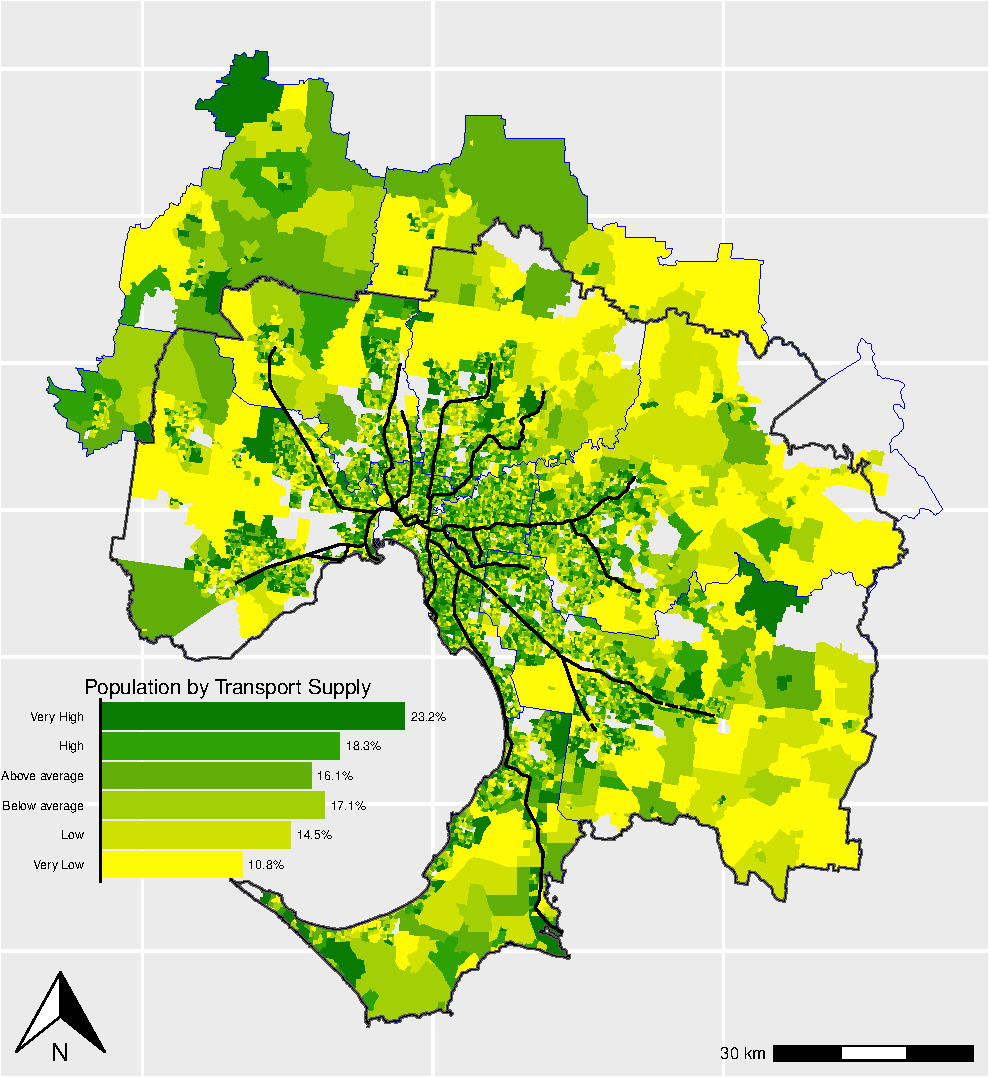
\includegraphics{ReynoldsCurrieQu2024_files/figure-latex/Greater_Melbourne_2021_social_needs-1.pdf}
\caption{Greater Melbourne 2021: Distribution of categories of composite
social need index scores, overlayed with: 2006 Greater Melbourne
boundary (black); SA4 boundaries (blue); and suburban railway lines
(dashed).}
\end{figure}

Figure \ref{fig:Greater_Melbourne_2021_social_needs} shows the
distribution of categories of social need index scores across Greater
Melbourne for 2021\footnote{A map for 2016 is included in the Appendix
  as Figure \ref{fig:Greater_Melbourne_2016_social_needs_appendix}}.
This is analogous to the 2006 map shown in Figure
\ref{fig:Currie_map_SI}(b) although, as discussed in the methodology
section above, it was not possible to exactly replicate the
\citet{currie2010identifying} social needs scoring approach due to
changes in how census results are reported. In general, the spatial
grouping of different levels of social need appears less consistently
grouped in 2021 than in 2006, although this may be an artifact of the
shift to SA1s from CCDs\footnote{CCDs were originally devised to group
  the approximately 200 dwellings allocated to each individual census
  collector, whereas SA1s were introduced to be consistent in population
  (200 to 800 people, averaging 400) and character
  \citep{ABS_SA1s_CCDs}.}.

\subsubsection{Needs-gap}\label{needs-gap}

\begin{figure}
\centering
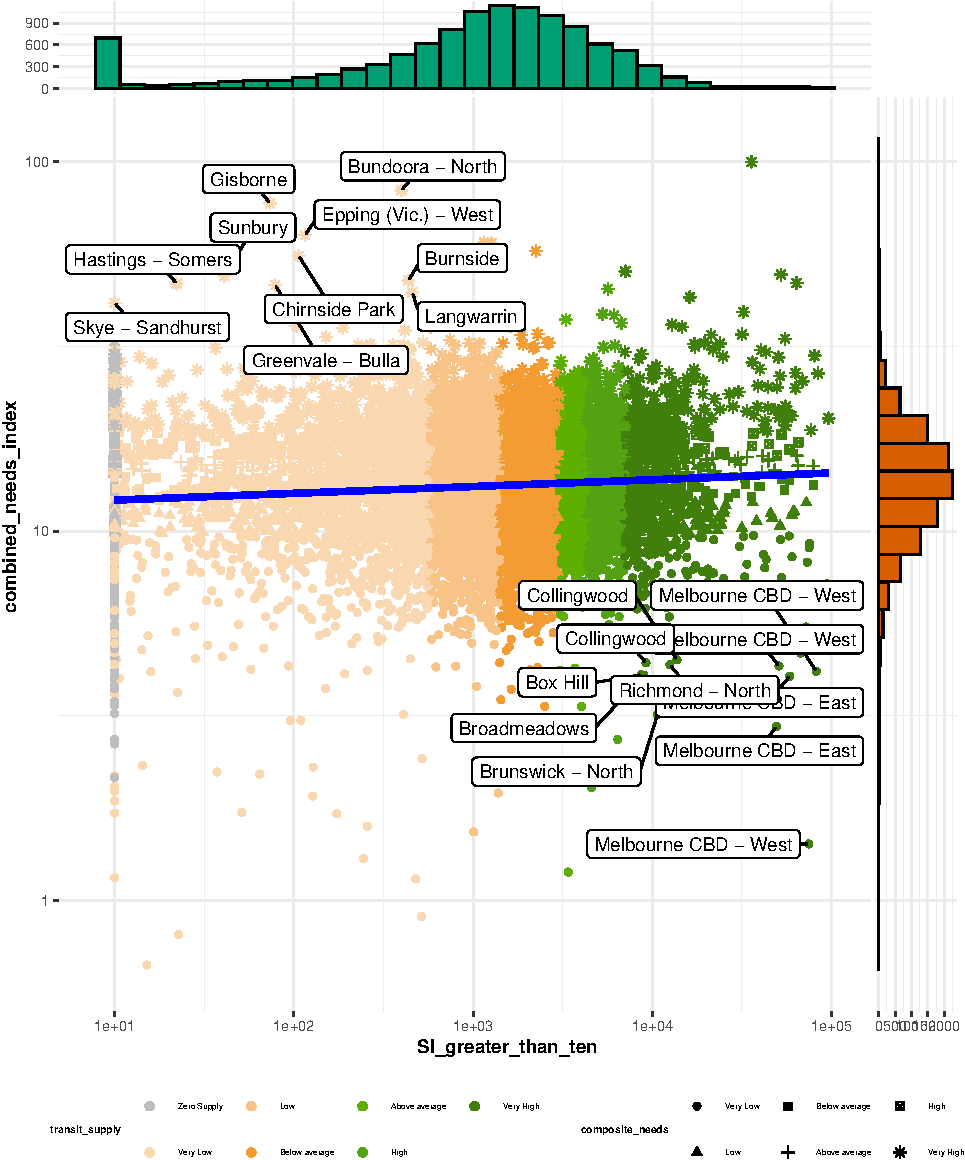
\includegraphics{ReynoldsCurrieQu2024_files/figure-latex/Greater_Melbourne_2021_needs_gap_scatterplot_figure-1.pdf}
\caption{Greater Melbourne 2021, SI and Combined Needs Index scores,
with SI scores \textless{} 10 rounded up to equal 10 to improve
clarity.}
\end{figure}

Figure \ref{fig:Greater_Melbourne_2021_needs_gap_scatterplot_figure}
shows social needs and SI scores for 2021\footnote{To improve the
  clarity of the figure, SI scores less than 10 have been adjusted to
  equal 10. As well, those SA1s with combinations of Zero or Very Low
  Transport Supply and (especially) high needs scores (more than 40); or
  Very High supply and Very Low needs scores (less than 4.5) have been
  labelled with their SA2 name, so as to given an indication of which
  suburbs of Melbourne are at each of the extremes. A similar plot for
  2016 is shown in the Appendix.}. This is analogous to the 2006 plot
shown in Figure 1(c). As might be expected, the (labeled) SA1s with
particularly low needs scores and Very High supply are mostly in inner
parts of the city\footnote{CBD, Richmond and Collingwood. Although
  Broadmeadows and Box Hill are notable exceptions, being located on
  rail lines in the middle to outer suburbs}, while those with
particularly high needs and Very Low supply are in the outer suburbs.
There is a significant, but only weakly positive correlation between the
SI and Combined Needs Index scores for both 2016 (\(r(11136) = .06\),
\(p < .001\), \(r_s =.07\), \(p < .001\)) and 2021 (\(r(11136) = .06\),
\(p < .001\), \(r_s =.07\), \(p < .001\))

Differences in the share of SA1s in each Transport Supply category
across different Combined Needs Index categories are statistically
significant in 2016 (\(\chi^2(30, N = 9964) = 264.26\), \(p < .001\))
and 2021 (\(\chi^2(30, N = 11138) = 133.51\), \(p < .001\) )\footnote{See
  Appendix for tables by SA1.}. Tables
\ref{tab:Greater_Melbourne_2016_needs_gap_population_table} and
\ref{tab:Greater_Melbourne_2021_needs_gap_population_table} compare the
populations within each Transport Supply and Combined Needs Index
grouping for 2016 and 2021. In 2016 301,743 people lived within SA1s
that had Zero or Very Low Transport Supply, but Very High social needs
(6.7\% of the total population). By 2021 this had increased to 333,887
people (+11\%, 6.7\% of the total population). These compare to the
139,004 people reported in \citet{currie2010identifying} for 2006 (4.2\%
of the population).

\begin{figure}
\centering
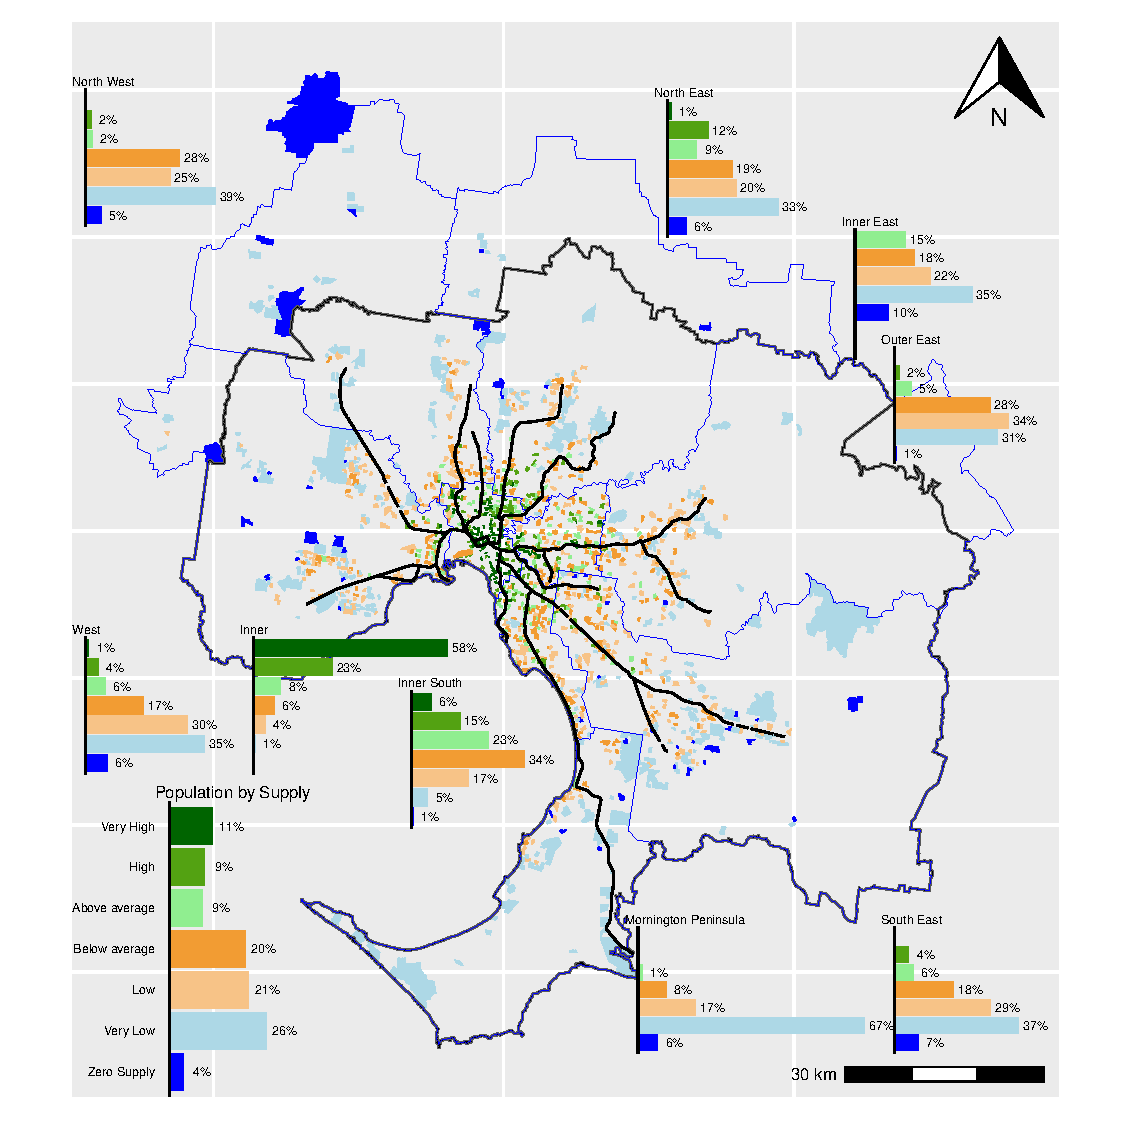
\includegraphics{ReynoldsCurrieQu2024_files/figure-latex/Greater_Melbourne_2021_needs_gap_map_figure-1.pdf}
\caption{Greater Melbourne 2021: Very High needs SA1s (only) Transport
Supply groupings,}
\end{figure}

Figure \ref{fig:Greater_Melbourne_2021_needs_gap_map_figure} shows SA1
zones in Greater Melbourne with Very High transport needs, but Very Low
or Zero Transport Supply for 2021, which is analogous to the 2006
distribution shown in Figure \ref{fig:Currie_map_SI}(d). Comparison
suggests that areas with larger gaps between social needs and transport
supply continue to be mostly in the outer areas of Melbourne, but this
appears complicated by the larger number of SA1s than CCDs\footnote{In
  that Figure \ref{fig:Greater_Melbourne_2021_needs_gap_map_figure}
  appears to show more (smaller) areas with Very High transport needs,
  but Very Low or Zero Transport Supply. This includes areas in the
  West, North West, North East and South East SA4s, whereas in 2006
  these parts of Melbourne did not appear to have large gaps between
  need and supply.}.

\subsubsection{Needs-gap and service level
changes}\label{needs-gap-and-service-level-changes}

\begin{table}

\caption{\label{tab:Greater_Melbourne_2016_needs_gap_SA4_service_change}Greater Melbourne: 2016 residents living in areas with Very High needs but Very Low or Zero supply, by SA4 and change in SI by 2021}
\centering
\fontsize{8}{10}\selectfont
\begin{tabular}[t]{>{\raggedright\arraybackslash}p{2.5cm}|>{\raggedleft\arraybackslash}p{1cm}|>{\raggedleft\arraybackslash}p{1cm}|>{\raggedleft\arraybackslash}p{1cm}|>{\raggedleft\arraybackslash}p{1cm}|>{\raggedleft\arraybackslash}p{1cm}|>{\raggedleft\arraybackslash}p{1cm}|>{\raggedleft\arraybackslash}p{1cm}|>{\raggedright\arraybackslash}p{1cm}|>{\raggedleft\arraybackslash}p{1.25cm}}
\hline
Change & Inner & Inner South & North East & North West & Outer East & South East & West & M'ton Pen. & Total\\
\hline
New or 30\%+ & 0.0\%     (0) & 0.5\% (1,512) & 3.6\% (10,928) & 7.2\% (21,707) & 0.0\%      (0) & 15.0\% (45,117) & 10.8\% (32,552) & 1.8\%  (5,342) & 38.8\% (117,158)\\
\hline
Increased 1 to 30\% & 0.2\%   (568) & 0.2\%   (648) & 3.4\% (10,172) & 3.0\%  (8,973) & 1.9\%  (5,843) & 6.5\% (19,533) & 7.6\% (22,823) & 2.1\%  (6,188) & 24.8\%  (74,748)\\
\hline
Within 1\% & 0.2\%   (546) & 0.4\% (1,271) & 1.9\%  (5,639) & 0.3\%    (953) & 4.8\% (14,489) & 5.3\% (15,974) & 4.1\% (12,378) & 4.1\% (12,421) & 21.1\%  (63,671)\\
\hline
Reduced, withdrawn, never & 0.0\%     (0) & 0.8\% (2,473) & 4.3\% (13,064) & 0.6\%  (1,878) & 1.2\%  (3,619) & 1.9\%  (5,835) & 3.9\% (11,773) & 2.5\%  (7,524) & 15.3\%  (46,166)\\
\hline
Total & 0.4\% (1,114) & 2.0\% (5,904) & 13.2\% (39,803) & 11.1\% (33,511) & 7.9\% (23,951) & 28.7\% (86,459) & 26.4\% (79,526) & 10.4\% (31,475) & 100.0\% (301,743)\\
\hline
\end{tabular}
\end{table}

\begin{figure}
\centering
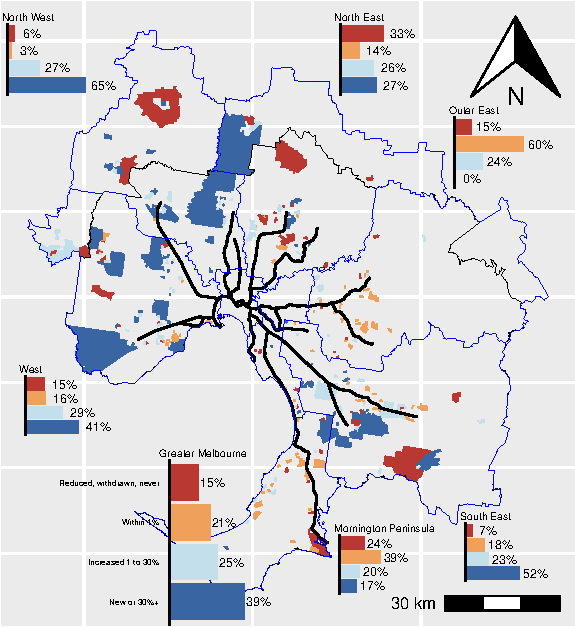
\includegraphics{ReynoldsCurrieQu2024_files/figure-latex/Greater_Melbourne_2016_needs_gap_SA4_service_change-1.pdf}
\caption{Greater Melbourne: change in transit supply between 2016 and
2021 for SA1s with Very High needs but Very Low or Zero supply in 2016}
\end{figure}

Figure \ref{fig:Greater_Melbourne_2016_needs_gap_SA4_service_change}
shows the change in transit supply between 2016 and 2021 for SA1s with
Very High needs but Very Low or Zero supply in 2016. There is a
statistically significant variation across the non-Inner SA4s\footnote{Categories
  of change in service level collapsed and the Inner, Inner East and
  Inner South SA4s removed to meet assumption of the chi-square test.}
\(\chi^2(15) = 92.59\), \(p < .001\). Table
\ref{tab:Greater_Melbourne_2016_needs_gap_SA4_service_change} shows how
much the transit service level changed for populations living in SA1s
with Very High needs but Very Low or Zero supply in 2016 by SA4. Service
levels had increased by 2021 for most of those living in Very High needs
but Very Low or Zero supply SA1s in 2016 in the North West (92\%, 30,680
people), South East (75\%, 64,650 people), the West (70\%, 55,375
people) and North East (53\%, 21,100 people). However, services had been
reduced or withdrawn, or were never present for 33\% of people living in
SA1s with Very High needs and Very Low or Zero supply in 2016 in the
North East (13,064people), 24\% of people living in SA1s with Very High
needs and Very Low or Zero supply in 2016 in the Mornington Peninsula
(7,524 people), 15\% in the West (11,773 people) and 15\% of people
living in SA1s with Very High needs and Very Low or Zero supply in 2016
in the Outer East (3,619 people).

\section{Discussion}\label{discussion}

This research was motivated by a lack of software tools to analyse gaps
between social needs for transport and the amount of transit provided,
and a need to better understand how spatial patterns might have changed
since the original development of this methodology in the early 2000s.
The needs-gaps approach was suggested to be ``substantially more useful
than the presentation of anecdotal evidence, which is the most common
means of identifying transport needs in local transport studies
throughout the world'' \citep{currie2010identifying}, yet this technique
does not appear to have been adopted in practice or received much
further attention from researchers. The research reported in this paper,
therefore, is important because it may help bridge gaps between research
(where the needs-gap approach and SI formulation was developed) and the
real world of transport planning, advocacy, professional practice and
politics (where decisions are made about where transit services are
needed or need improving).

As discussed in Section 2, there are many transit metrics available, but
these may be impossible to calculate independently or complicated to use
for the purposes of communicating with the public, decision-makers or
other stakeholders. The SI has the advantage of combining accessibility
and service frequency into a single measure, which is relatively simple
to understand and can even be calculated by hand for smaller networks.
The gtfstools R package developed in this research may make it possible
for practitioners to apply the SI calculation across even relatively
large transit networks, such as that of Greater Melbourne, with a GTFS
feed and some computer time. While the tool is not yet at a download,
point and click level of usability, it is open source and publicly
available and so may make assessing transit service levels and network
change proposals with respect to social needs for transport more widely
achievable.

The maps, graphs, tables and other outputs presented in this paper also
demonstrate the range of analysis that might be possible using this
package. Longitudinal comparison of transit service levels has been
shown in aggregate (Table
\ref{tab:Greater_Melbourne_CCDs_SA1_population}), by population across
sub-areas (in comparing Tables
\ref{tab:Greater_Melbourne_population_2016_by_SA4} and
\ref{tab:Greater_Melbourne_population_2021_by_SA4}) and mapped (Figure
\ref{fig:Greater_Melbourne_2016_2021_ratio_map}). Visual display of gaps
between social needs and Transport Supply how also been shown through
scatterplots (Figures
\ref{fig:Greater_Melbourne_2016_needs_gap_scatterplot} and
\ref{fig:Greater_Melbourne_2021_needs_gap_scatterplot}) and mapping
(Figures \ref{fig:Greater_Melbourne_2016_needs_gap_map} and
\ref{fig:Greater_Melbourne_2021_needs_gap_map}). Such outputs,
especially if produced at the spatial level of a neighbourhood, council
ward or electoral division, might provide an opportunity for advocates
and professionals within transport planning to identify and easily
demonstrate to the public, politician and other stakeholders which
spatial areas might benefit from increasing transit funding and where
funds might best be directed. The map shown in Figure
\ref{fig:Greater_Melbourne_2016_needs_gap_SA4_service_change}
demonstrates how the needs-gap analysis approach, in conjunction with a
comparison of service levels through time, cam be used to show how
things have changed for those residents who had Very High transport
needs, but Very Low or Zero Supply. Such maps might provide evidence for
those living in areas with high needs, but where service levels have
moved in the wrong direction, such as appears to be the case for
13,064people living in the North East (24\%) and 7,524 people living in
the Mornington Peninsula in SA1s with Very High needs and Very Low or
Zero supply in 2016 who saw their transit service reduced or withdrawn
by 2021, or who never had any transit at all.

The changes by 2021, however, appear to have been mostly positive for
the 39,803people living in the South East SA4 in 2016 in SA1s with Very
High needs and Very Low or Zero supply. Table
\ref{tab:Greater_Melbourne_2016_needs_gap_SA4_service_change} indicates
that 75\%) of them would have received at least a one percent increase
in transit service levels, while Figure
\ref{fig:Greater_Melbourne_2016_needs_gap_SA4_service_change} suggests
that areas around Cranbourne have seen substaintial service increases
(30\%+) or the introduction of new services (dark blue). This part of
Greater Melbourne has received attention from previous research reported
in \citet{delbosc2015impact}, which looked at bus services in new
developments and included a case study of the Selandra Rise planned
estate, east of Cranbourne. This study explored the impact of the, then
newly introduced, 798 bus route (Figure \ref{fig:Bus_798}. The route was
reported as having around 2,500 boardings per week and being used by at
least one person in 35 percent of households within the Selandra Rise
Estate, despite it not penetrating fully into the development and only
20 percent of the estate's footprint being within 400 metres of the
route. Findings suggested that: the route was ``performing an important
`social transit' function''; that ``those who do use the bus use it very
frequently (88 percent (of riders) at least a few days a week)''; ``Most
bus riders were young and could not drive or had no car available,
making them quite reliant on the bus'', and that it ``frees up the time
of other household members who would have had to provide lifts''
\citep[p.10]{delbosc2015impact}. Figure \ref{fig:Selandra_rise} revisits
the Selandra Rise Estate, showing Transport Supply in 2016 and 2021, and
changes in SI score for those SA1s that had Very High social needs, but
Very Low or Zero Transport Supply in 2016.

\begin{figure}

{\centering \subfloat[Bus Route 798 as originally introduced in 2014 (Source: Delbosc et al (2015))\label{fig:Bus_798-1}]{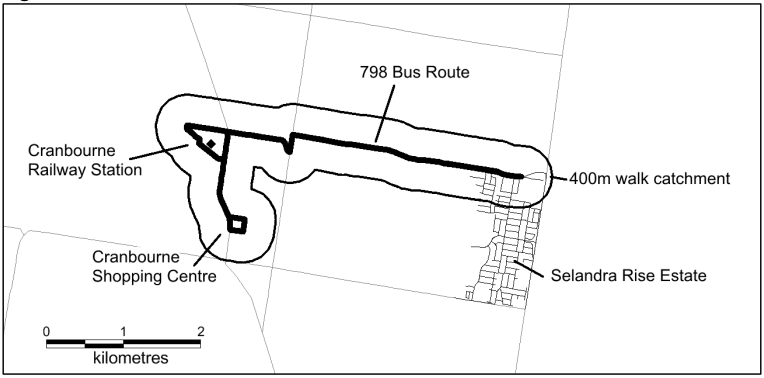
\includegraphics[width=0.5\linewidth]{graphics/Route798} }\subfloat[Current (2024) route map (Source: PTV)\label{fig:Bus_798-2}]{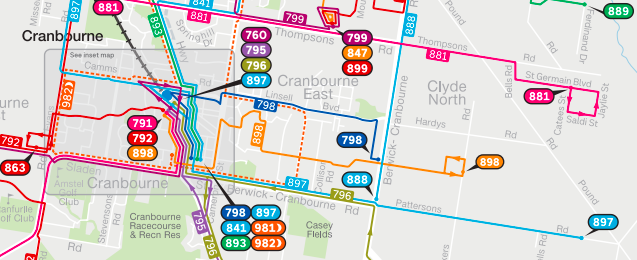
\includegraphics[width=0.5\linewidth]{graphics/Selandra_Rise} }

}

\caption{Cranbourne and Selandra Rise}\label{fig:Bus_798}
\end{figure}

\begin{figure}

{\centering \subfloat[Transport Supply by SA1: 2016\label{fig:Selandra_rise-1}]{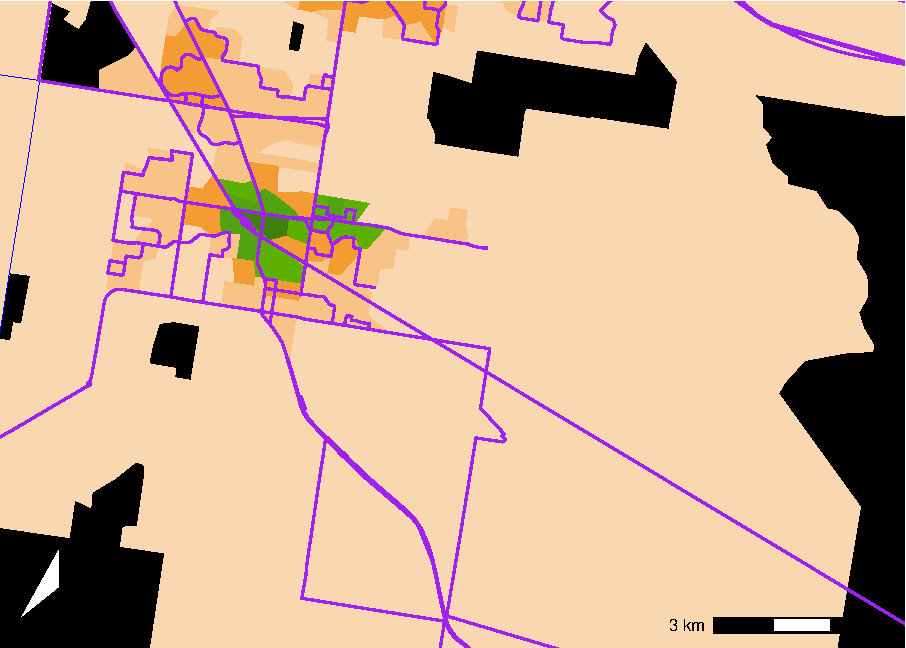
\includegraphics{ReynoldsCurrieQu2024_files/figure-latex/Selandra_rise-1} }\subfloat[Transport Supply by population: 2016\label{fig:Selandra_rise-2}]{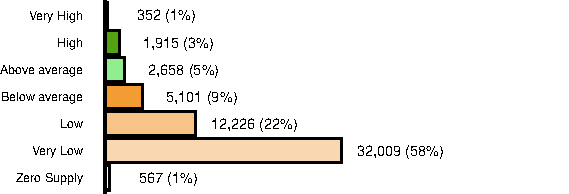
\includegraphics{ReynoldsCurrieQu2024_files/figure-latex/Selandra_rise-2} }\newline\subfloat[Transport Supply by SA1: 2021\label{fig:Selandra_rise-3}]{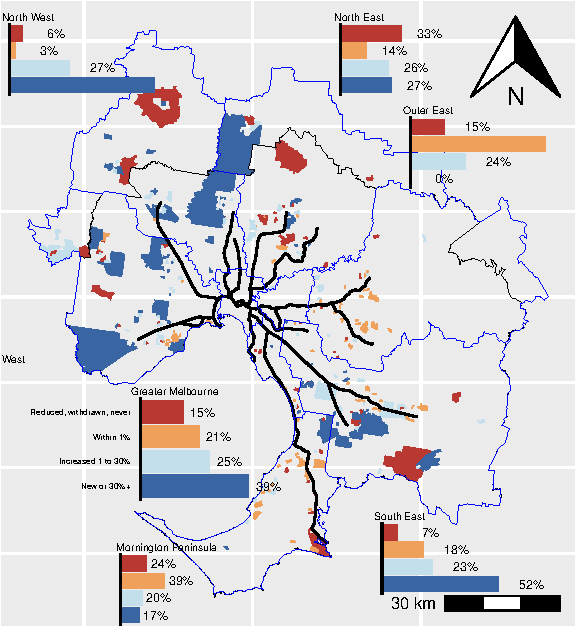
\includegraphics{ReynoldsCurrieQu2024_files/figure-latex/Selandra_rise-3} }\subfloat[Transport Supply by population: 2021\label{fig:Selandra_rise-4}]{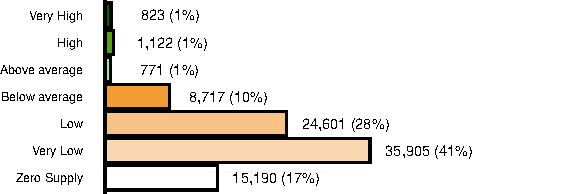
\includegraphics{ReynoldsCurrieQu2024_files/figure-latex/Selandra_rise-4} }\newline\subfloat[Change in SI score between 2016 and 2021 by SA1 (2021 boundaries)\label{fig:Selandra_rise-5}]{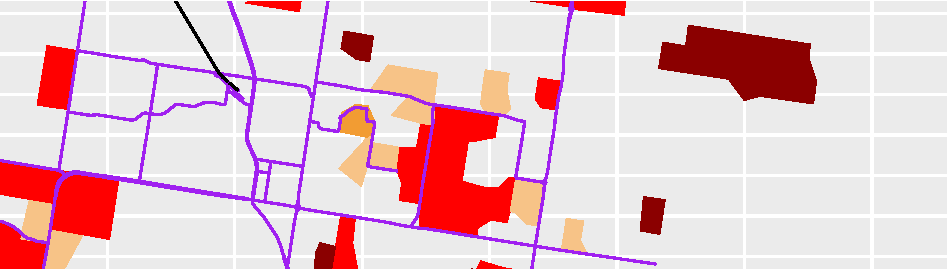
\includegraphics{ReynoldsCurrieQu2024_files/figure-latex/Selandra_rise-5} }\subfloat[Change in SI score between 2016 and 2021, by 2021 population\label{fig:Selandra_rise-6}]{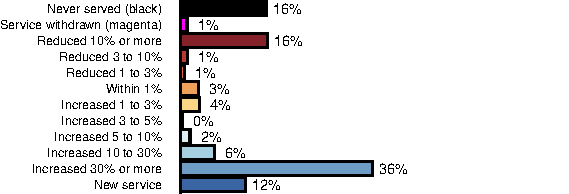
\includegraphics{ReynoldsCurrieQu2024_files/figure-latex/Selandra_rise-6} }\newline\subfloat[Social Need by SA1: 2021\label{fig:Selandra_rise-7}]{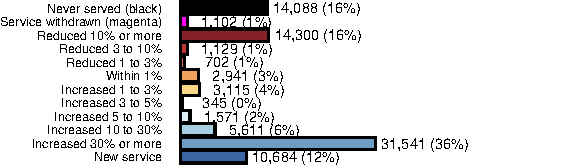
\includegraphics{ReynoldsCurrieQu2024_files/figure-latex/Selandra_rise-7} }\subfloat[Social Need by population: 2021\label{fig:Selandra_rise-8}]{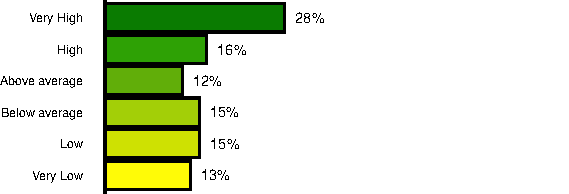
\includegraphics{ReynoldsCurrieQu2024_files/figure-latex/Selandra_rise-8} }\newline\subfloat[Needs-gap: SA1s with Very High transport needs in 2021, by Transport Supply\label{fig:Selandra_rise-9}]{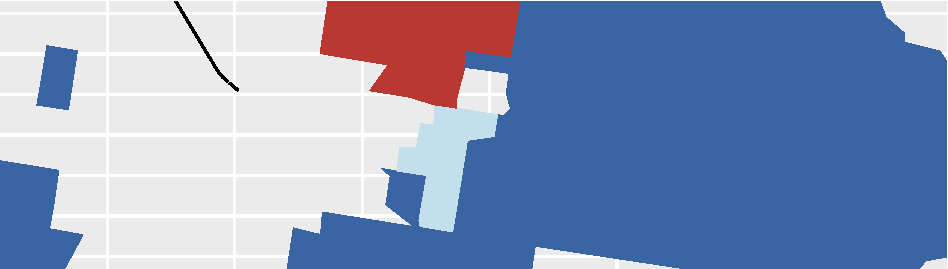
\includegraphics{ReynoldsCurrieQu2024_files/figure-latex/Selandra_rise-9} }\subfloat[Needs-gap: population with Very High transport needs in 2021, by Transport Supply\label{fig:Selandra_rise-10}]{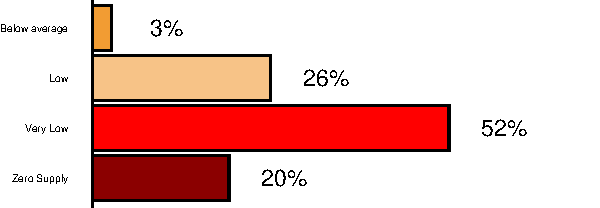
\includegraphics{ReynoldsCurrieQu2024_files/figure-latex/Selandra_rise-10} }\newline

}

\caption{Cranbourne and the Selandra Rise Estate}\label{fig:Selandra_rise}
\end{figure}

Various transit routes appear to have been added to the area surrounding
the Selandra Rise Estate between 2016 (Figure
\ref{fig:Selandra_rise}(a), 2021 (b) and 2024 (d)\footnote{After 2016
  Route 798 was adjusted to penetrate into the estate, and Route 888 was
  added to provide a north-south connection along Berwick-Cranbourne
  Road.}. This appears to have been sufficient to shift some of the
estate into the Low Transport Supply category in 2021, up from Very Low
category in 2016.

Figure \ref{fig:Selandra_rise}(c), however, indicates that some of the
surrounding SA1s, however, still fall into the Very High needs and Very
Low or Zero supply social needs-gap category, including some SA1s that
have over 700 residents but did not have a transit service within 400
metres in either 2016 and 2021.\footnote{It appears that Route 898 has
  been added between 2021 and 2024, providing an additional east-west
  connection and coverage, suggesting that the ultimate transit network
  for the area was not yet implemented in 2021.}. Such mapping of SI
change, needs-gaps and route information, as in Figure
\ref{fig:Selandra_rise}, might provide an example of how social needs
could be given greater consideration in the planning of transit networks
in new subdivisions\footnote{For example, the maps suggest that areas in
  the vicinity of Casey Fields remain underserved. Revising Route 795 so
  as to service areas north of Ballarto Rd, perhaps instead of
  duplicating parts of Route 796, might be one option to increase
  coverage and provide some stops for residents living in areas that did
  not have an transit within 400 metres in either 2016 or 2021.}.

\section{Conclusions}\label{conclusions}

This paper has reported the development of a new R package containing
tools for identifying gaps between the social need for transport and the
service provided based on GTFS data. It has also demonstrated how this
package might be applied to the case of Greater Melbourne in 2016 and
2021, in the same manner in which \citet{currie2010identifying} applied
the analysis approach to Melbourne in 2006.

A motivation for this study was explore how spatial patterns related to
Transport Supply, need and gaps have changed in Melbourne since 2006. To
some extent the results indicate the challenges of making longitudinal
comparisons when there are changes in statistical geography. The shift
from CCDs to SA1s by the ABS appears to have allowed results to be
output here are a finer scale than in 2006, due to the generally smaller
size of SA1s and the way in which they are focused towards containing
consistent land use patterns within each zone. This contrasts to the
CCDs, which instead denoted the areas within which one census collector
operated. Unfortunately, this limits the extend to which the 2016 and
2021 results can be directly compared to those for 2006. However, it is
notable that the share of the population living in areas wtih Zero
Transport Supply grew with time from 2.5\% (85,423 residents) in 2006 to
2.9\% (131,619 residents) in 2016, and then again to 3.8\% (186,829
residents) in 2021. How much of the change between 2006 and 2016 relates
to the switch in statistical geography is unclear, but the difference
between 2016 and 2021 suggests that as time marches on more people and a
greater proportion of the population are living in areas where transit
stops are beyond typical walking access distance.

Compared to the 8.2\% (276,739) of Melbourne residents having Very High
needs but Low, Very Low or Zero Transport Supply in 2006 reported by
\citet{currie2010identifying} this study found equivalents of 11.2\%
(502,680 residents) in 2016 and 11.2\% ( 301,743 residents) in 2021.
Again, the 2016 and 2021 values may not directly comparable to those
from 2006 because of the statistical geography changes. However, these
findings might again suggest that the situation is moving in the wrong
direction, at least in Greater Melbourne.

\subsection{Limitations and future research
directions}\label{limitations-and-future-research-directions}

The extent to which the findings about Greater Melbourne can be
confidently generalised to other places (relating to the duality
criterion of case research) is a key question, which is not yet fully
answered. Fortunately, the widespread availability of GTFS datasets
together with the new gtfssupplyindex package means that it will be
easier to analyse other cases so as to better understand whether
Melbourne is representative. Exploring social needs-gaps in other
Australian cities is an immediate direction for future efforts
associated with this program of research. In the meantime, it would seem
prudent to be cautious as to making assumptions about whether shifts in
Melbourne are representative of everywhere else. The almost 50 percent
growth in population in Greater Melbourne between 2006 (3.4m) and 2021
(4.9m) may be more than is typical, although the low-density development
patterns in Greater Melbourne appear common elsewhere within and beyond
Australia, suggesting that the study's findings about widening gaps in
outer areas are likely to be generalisable. Melbourne is currently
building a new subway connection through the CBD and a second freeway
connection of its largest river, and various other rail and road
mega-projects are either in planning or recently completed. As such,
Melbourne might be an outlier as far as the share of government spending
going towards transport that is not focused on providing basic coverage
for those who cannot otherwise drive or increasing service levels for
those with the greatest social need for transit. That said, the
challenges related to building business cases, increasing subsidies and
otherwise introducing or increasing transit service in outer areas would
appear likely to be similar in Melbourne as to other places. Hence, it
might be confidentially expected that the overall patterns, of the
largest gaps between the social need for transport and the transit
supplied being in outer suburbs and away from suburban railway lines,
might be reasonably expected in other cities.

As well as making comparisons of Melbourne across 2006, 2016 and 2021,
this paper has expanded on the analysis approach developed in
\citet{Currie2003Hobart}, \citet{Currie2004Gap},
\citet{Currie2007Identifying} and \citet{currie2010identifying}. The
mapping of changes in SI scores (Figure
\ref{fig:Greater_Melbourne_2016_2021_ratio_map}) and how these changes
relate to transit routes and areas with large needs-gaps at a
neighbourhood (Figure \ref{fig:Selandra_rise}) might be of use to
transport planners, advocates, politicians and other decision-makers,
and others seeking to build legitimacy for the improvement or
introduction of basic transit service levels. It is heartening that the
Selandra Rise Estate, where \citet{delbosc2015impact} found that what
transit was initially implemented provided a very important social
function and that there was a community desire for greater levels of
service, now has more routes and higher service levels. However, Figure
\ref{fig:Selandra_rise} shows that there were similarly
under-or-never-served communities nearby in 2021, suggesting that the
timely introduction of transit service to new development areas
continues to be a challenge in parts of Melbourne. Further research
might seek to confirm the extent to which similar issues are evident in
other cities.

Overall, the research reported in this paper may help practitioners and
decision-makers more easily identify gaps between the social need for
transport and the transit supplied. \citet{currie2010identifying}
suggested that using the Supply Index and needs-gap analysis techniques
would be much preferable to anecdotal or other informal inputs to
decision-making, which are common in practice. The software package and
analysis approaches reported in this paper, enabling GTFS data to be
directly used as an input, may allow the social needs-gap approach to be
used more easily and more widely to target new and improved services to
where they are most needed by the community.

\section*{References}\label{references}
\addcontentsline{toc}{section}{References}

\section{Appendix}\label{appendix}

\begin{figure}

{\centering \subfloat[Melbourne (2006 extents), Transport Supply by CCD for the week starting the date of the 2016 census, overlayed with suburban railway lines (black) and inner, middle and outer suburban boundary\label{fig:Greater_Melbourne_CCD_2016_appendix-1}]{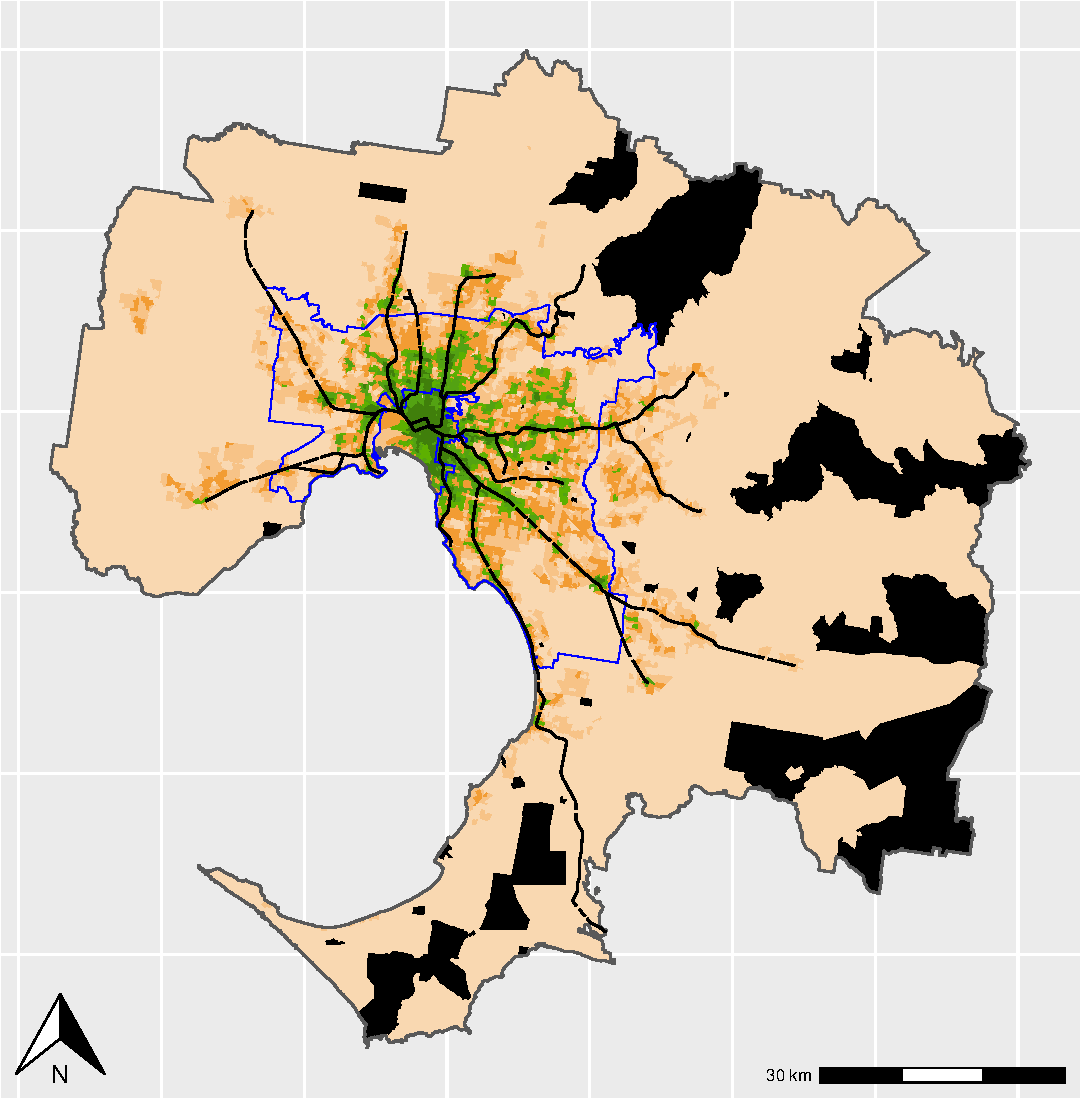
\includegraphics[width=0.5\linewidth]{ReynoldsCurrieQu2024_files/figure-latex/Greater_Melbourne_CCD_2016_appendix-1} }\subfloat[Melbourne (2006 extents), Transport Supply by CCD for the week starting the date of the 2021 census, overlayed with suburban railway lines (black) and inner, middle and outer suburban boundary\label{fig:Greater_Melbourne_CCD_2016_appendix-2}]{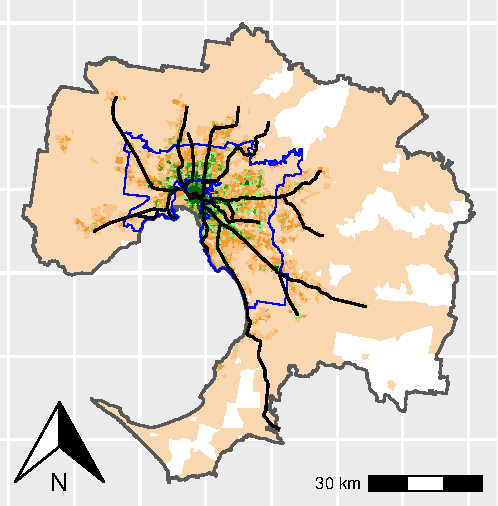
\includegraphics[width=0.5\linewidth]{ReynoldsCurrieQu2024_files/figure-latex/Greater_Melbourne_CCD_2016_appendix-2} }

}

\caption{Transport Supply Categories. Source: Currie (2010)}\label{fig:Greater_Melbourne_CCD_2016_appendix}
\end{figure}

\begin{table}

\caption{\label{tab:Greater_Melbourne_SA1_2016_by_SA4}Greater Melbourne 2016: SA1s in each Transport Supply category by SA4}
\centering
\fontsize{8}{10}\selectfont
\begin{tabular}[t]{>{\raggedright\arraybackslash}p{1.75cm}|>{\raggedleft\arraybackslash}p{1cm}|>{\raggedleft\arraybackslash}p{1cm}|>{\raggedleft\arraybackslash}p{1cm}|>{\raggedleft\arraybackslash}p{1cm}|>{\raggedleft\arraybackslash}p{1cm}|>{\raggedleft\arraybackslash}p{1cm}|>{\raggedleft\arraybackslash}p{1cm}|>{\raggedright\arraybackslash}p{1cm}|>{\raggedleft\arraybackslash}p{1cm}|>{\raggedleft\arraybackslash}p{1.25cm}}
\hline
Transport Supply & Inner & Inner East & Inner South & North East & North West & Outer East & South East & West & M'ton Pen. & Total\\
\hline
Zero Supply & 0.0\%     (0) & 0.0\%   (1) & 0.0\%   (5) & 0.5\%    (48) & 0.4\%  (43) & 0.4\%    (42) & 1.0\%   (101) & 0.2\%    (23) & 0.6\%  (63) & 3.2\%    (326)\\
\hline
Very Low & 0.1\%    (10) & 0.5\%  (50) & 0.7\%  (70) & 2.5\%   (257) & 2.1\% (215) & 5.0\%   (511) & 4.6\%   (473) & 3.7\%   (377) & 3.9\% (399) & 23.0\%  (2,362)\\
\hline
Low & 0.4\%    (44) & 0.9\%  (95) & 1.4\% (142) & 2.8\%   (288) & 2.4\% (243) & 3.2\%   (329) & 5.0\%   (518) & 5.3\%   (541) & 1.6\% (162) & 23.0\%  (2,362)\\
\hline
Below average & 1.0\%   (105) & 2.4\% (249) & 2.9\% (298) & 3.1\%   (319) & 2.2\% (231) & 2.8\%   (284) & 4.0\%   (411) & 3.9\%   (399) & 0.6\%  (66) & 23.0\%  (2,362)\\
\hline
Above average & 1.1\%   (111) & 1.8\% (186) & 1.8\% (184) & 1.0\%   (103) & 0.7\%  (70) & 0.6\%    (60) & 1.1\%   (114) & 1.2\%   (122) & 0.1\%   (9) & 9.3\%    (959)\\
\hline
High & 2.7\%   (279) & 1.7\% (175) & 1.6\% (168) & 1.0\%   (107) & 0.3\%  (31) & 0.4\%    (39) & 0.7\%    (70) & 0.8\%    (86) & 0.0\%   (4) & 9.3\%    (959)\\
\hline
Very High & 6.7\%   (685) & 0.8\%  (86) & 0.7\%  (75) & 0.4\%    (41) & 0.1\%   (7) & 0.0\%     (1) & 0.2\%    (16) & 0.5\%    (48) & 0.0\%   (0) & 9.3\%    (959)\\
\hline
Total & 12.0\% (1,234) & 8.2\% (842) & 9.2\% (942) & 11.3\% (1,163) & 8.2\% (840) & 12.3\% (1,266) & 16.6\% (1,703) & 15.5\% (1,596) & 6.8\% (703) & 100.0\% (10,289)\\
\hline
\end{tabular}
\end{table}

\begin{figure}
\centering
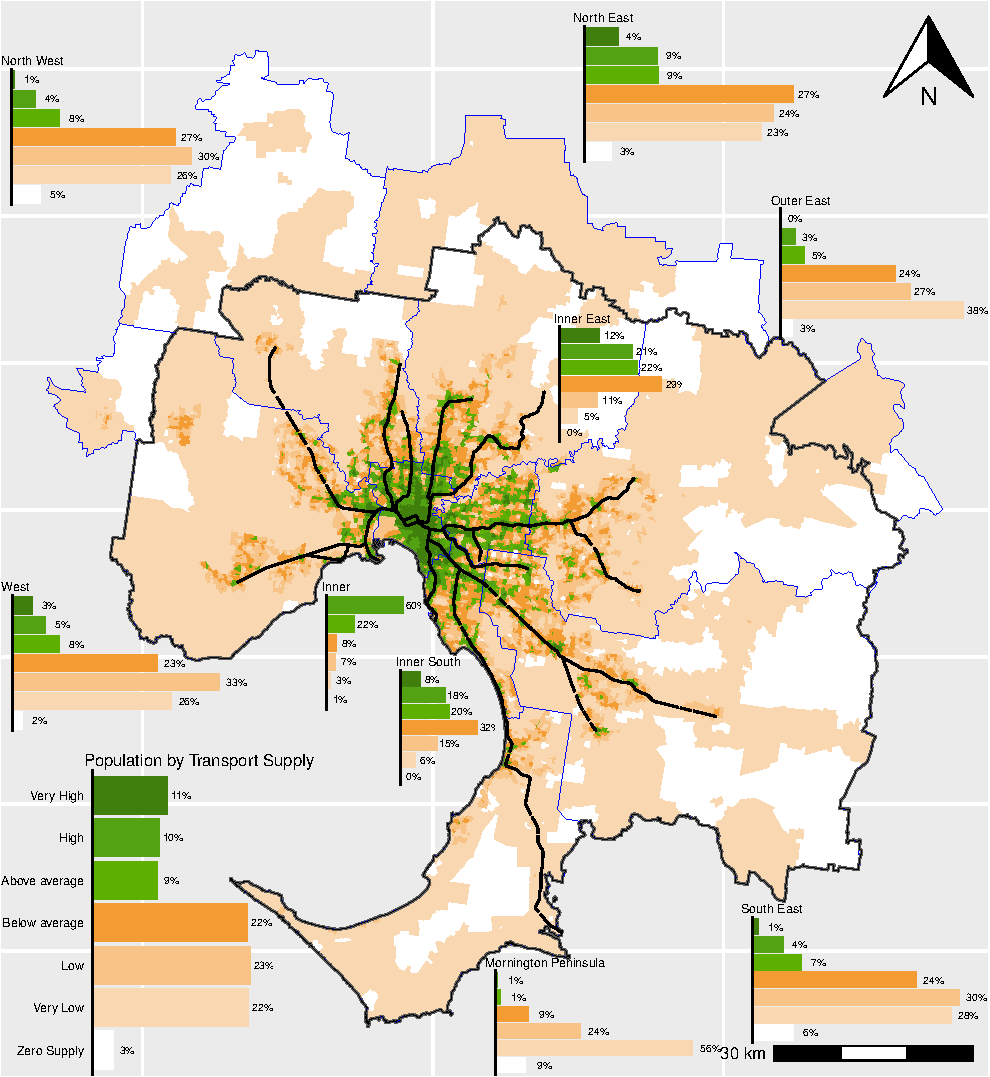
\includegraphics{ReynoldsCurrieQu2024_files/figure-latex/Greater_Melbourne_SA12016_plot_appendix-1.pdf}
\caption{Greater Melbourne 2016: Transport Supply by SA1, overlayed with
suburban rail network (black), SA4 boundaries (blue) and 2006 Melbourne
extents (black)}
\end{figure}

\begin{table}

\caption{\label{tab:Greater_Melbourne_SA1_2021_by_SA4}Greater Melbourne 2016: SA1s in each Transport Supply category by SA4}
\centering
\fontsize{8}{10}\selectfont
\begin{tabular}[t]{>{\raggedright\arraybackslash}p{1.75cm}|>{\raggedleft\arraybackslash}p{1cm}|>{\raggedleft\arraybackslash}p{1cm}|>{\raggedleft\arraybackslash}p{1cm}|>{\raggedleft\arraybackslash}p{1cm}|>{\raggedleft\arraybackslash}p{1cm}|>{\raggedleft\arraybackslash}p{1cm}|>{\raggedleft\arraybackslash}p{1cm}|>{\raggedright\arraybackslash}p{1cm}|>{\raggedleft\arraybackslash}p{1cm}|>{\raggedleft\arraybackslash}p{1.25cm}}
\hline
Transport Supply & Inner & Inner East & Inner South & North East & North West & Outer East & South East & West & M'ton Pen. & Total\\
\hline
Zero Supply & 0.0\%     (0) & 0.0\%   (1) & 0.0\%   (5) & 0.6\%    (71) & 0.5\%  (55) & 0.4\%    (44) & 1.2\%   (142) & 1.0\%   (112) & 0.5\%  (59) & 4.3\%    (489)\\
\hline
Very Low & 0.1\%    (13) & 0.5\%  (54) & 0.5\%  (63) & 2.7\%   (307) & 2.2\% (254) & 4.6\%   (523) & 5.0\%   (576) & 4.4\%   (504) & 3.5\% (398) & 23.4\%  (2,692)\\
\hline
Low & 0.4\%    (48) & 0.9\% (108) & 1.3\% (147) & 2.8\%   (322) & 2.4\% (279) & 3.2\%   (368) & 5.3\%   (608) & 5.7\%   (653) & 1.4\% (158) & 23.4\%  (2,691)\\
\hline
Below average & 1.1\%   (130) & 2.7\% (310) & 2.9\% (333) & 3.2\%   (363) & 2.6\% (297) & 2.3\%   (261) & 4.1\%   (470) & 3.8\%   (437) & 0.8\%  (90) & 23.4\%  (2,691)\\
\hline
Above average & 1.2\%   (137) & 1.4\% (160) & 1.8\% (210) & 0.9\%   (101) & 0.5\%  (63) & 0.4\%    (49) & 1.0\%   (114) & 1.1\%   (128) & 0.1\%  (13) & 8.5\%    (975)\\
\hline
High & 3.0\%   (345) & 1.5\% (172) & 1.4\% (161) & 0.8\%    (95) & 0.2\%  (22) & 0.3\%    (29) & 0.5\%    (55) & 0.8\%    (93) & 0.0\%   (2) & 8.5\%    (974)\\
\hline
Very High & 6.6\%   (763) & 0.6\%  (65) & 0.5\%  (57) & 0.2\%    (26) & 0.0\%   (5) & 0.0\%     (0) & 0.2\%    (19) & 0.3\%    (40) & 0.0\%   (0) & 8.5\%    (975)\\
\hline
Total & 12.5\% (1,436) & 7.6\% (870) & 8.5\% (976) & 11.2\% (1,285) & 8.5\% (975) & 11.1\% (1,274) & 17.3\% (1,984) & 17.1\% (1,967) & 6.3\% (720) & 100.0\% (11,487)\\
\hline
\end{tabular}
\end{table}

\begin{table}

\caption{\label{tab:Greater_Melbourne_2016_2021_ratio_SA1_table}Greater Melbourne: Share of 2021 SA1s by change in transit service (2016 vs 2021) by SA4 region}
\centering
\fontsize{8}{10}\selectfont
\begin{tabular}[t]{>{\raggedright\arraybackslash}p{1.75cm}|>{\raggedleft\arraybackslash}p{1cm}|>{\raggedleft\arraybackslash}p{1cm}|>{\raggedleft\arraybackslash}p{1cm}|>{\raggedleft\arraybackslash}p{1cm}|>{\raggedleft\arraybackslash}p{1cm}|>{\raggedleft\arraybackslash}p{1cm}|>{\raggedleft\arraybackslash}p{1cm}|>{\raggedright\arraybackslash}p{1cm}|>{\raggedleft\arraybackslash}p{1cm}|>{\raggedleft\arraybackslash}p{1.25cm}}
\hline
Change & Inner & Inner East & Inner South & North East & North West & Outer East & South East & West & M'ton Pen. & Total\\
\hline
New service & 0.0\%     (0) & 0.0\%   (0) & 0.0\%   (0) & 0.2\%    (20) & 0.7\%  (79) & 0.0\%     (1) & 1.0\%   (113) & 0.8\%    (87) & 0.1\%   (6) & 2.7\%    (306)\\
\hline
Increased 30\% or more & 0.0\%     (5) & 0.0\%   (1) & 0.7\%  (83) & 0.9\%   (107) & 1.5\% (173) & 0.1\%    (10) & 2.6\%   (293) & 2.5\%   (290) & 1.3\% (154) & 9.7\%  (1,116)\\
\hline
Increased 10 to 30\% & 0.9\%   (104) & 0.1\%   (7) & 0.9\%  (99) & 0.8\%    (95) & 1.2\% (133) & 0.5\%    (54) & 1.5\%   (173) & 2.0\%   (231) & 0.4\%  (49) & 8.2\%    (945)\\
\hline
Increased 5 to 10\% & 1.4\%   (166) & 0.2\%  (28) & 1.0\% (120) & 0.8\%    (90) & 0.7\%  (75) & 0.6\%    (69) & 1.0\%   (120) & 2.0\%   (233) & 0.2\%  (23) & 8.0\%    (924)\\
\hline
Increased 3 to 5\% & 1.6\%   (185) & 0.5\%  (58) & 0.6\%  (71) & 1.3\%   (147) & 1.1\% (122) & 0.5\%    (63) & 0.9\%   (104) & 1.8\%   (210) & 0.3\%  (32) & 8.6\%    (992)\\
\hline
Increased 1 to 3\% & 2.4\%   (281) & 1.3\% (152) & 1.2\% (142) & 1.9\%   (214) & 0.9\% (107) & 0.9\%   (101) & 1.5\%   (176) & 2.4\%   (271) & 0.7\%  (76) & 13.2\%  (1,520)\\
\hline
Within 1\% & 2.5\%   (286) & 3.9\% (444) & 1.9\% (223) & 2.6\%   (295) & 1.2\% (138) & 5.8\%   (661) & 5.4\%   (620) & 3.0\%   (347) & 2.3\% (261) & 28.5\%  (3,275)\\
\hline
Reduced 1 to 3\% & 1.0\%   (114) & 0.8\%  (94) & 0.5\%  (63) & 0.8\%    (89) & 0.3\%  (32) & 0.8\%    (92) & 0.7\%    (77) & 0.4\%    (44) & 0.4\%  (42) & 5.6\%    (647)\\
\hline
Reduced 3 to 10\% & 1.8\%   (212) & 0.5\%  (61) & 0.9\% (100) & 0.9\%   (105) & 0.2\%  (28) & 0.9\%   (102) & 0.5\%    (58) & 0.7\%    (79) & 0.1\%  (15) & 6.6\%    (760)\\
\hline
Reduced 10\% or more & 0.7\%    (83) & 0.2\%  (24) & 0.6\%  (70) & 0.5\%    (52) & 0.3\%  (33) & 0.7\%    (77) & 0.9\%   (108) & 0.5\%    (63) & 0.0\%   (3) & 4.5\%    (513)\\
\hline
Service withdrawn (magenta) & 0.0\%     (0) & 0.0\%   (0) & 0.0\%   (0) & 0.0\%     (4) & 0.0\%   (1) & 0.0\%     (3) & 0.0\%     (3) & 0.0\%     (4) & 0.0\%   (0) & 0.1\%     (15)\\
\hline
Never served (black) & 0.0\%     (0) & 0.0\%   (1) & 0.0\%   (5) & 0.6\%    (67) & 0.5\%  (54) & 0.4\%    (41) & 1.2\%   (139) & 0.9\%   (108) & 0.5\%  (59) & 4.1\%    (474)\\
\hline
Total & 12.5\% (1,436) & 7.6\% (870) & 8.5\% (976) & 11.2\% (1,285) & 8.5\% (975) & 11.1\% (1,274) & 17.3\% (1,984) & 17.1\% (1,967) & 6.3\% (720) & 100.0\% (11,487)\\
\hline
\end{tabular}
\end{table}

\begin{figure}
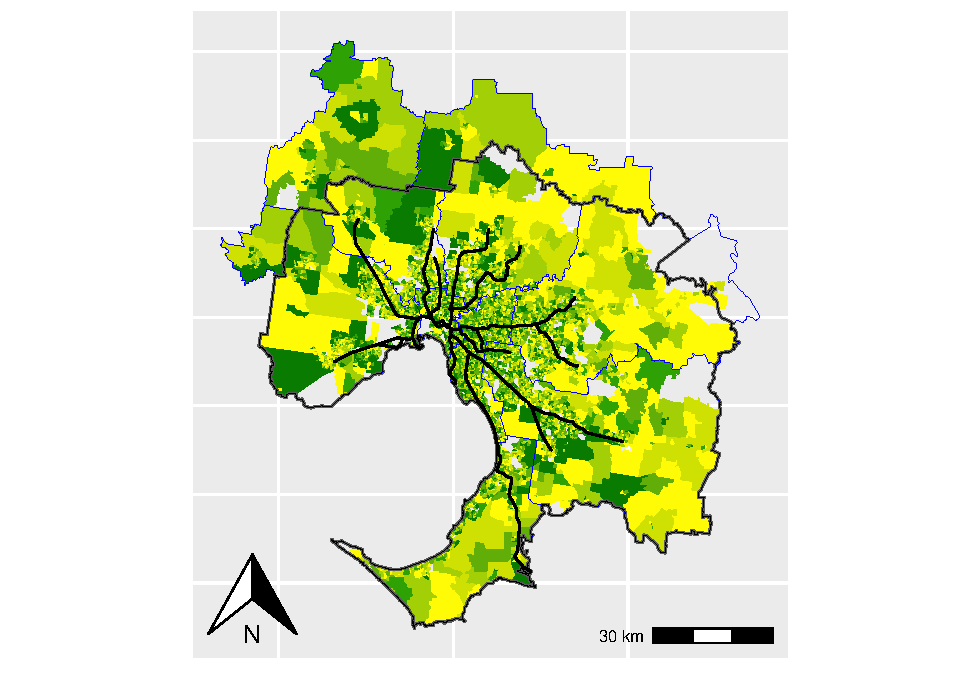
\includegraphics[width=0.9\linewidth]{ReynoldsCurrieQu2024_files/figure-latex/Greater_Melbourne_2016_social_needs_appendix-1} \caption{Distribution of categories of composite social need index scores in 2016 (left) and 2021 (right), overlayed with: 2006 Greater Melbourne boundary (black); middle/outer and inner/middle suburb boundaries (grey); and suburban railway lines (dashed).}\label{fig:Greater_Melbourne_2016_social_needs_appendix}
\end{figure}

\begin{table}

\caption{\label{tab:Greater_Melbourne_2016_needs_gap_zones}Greater Melbourne 2016, SA1s within each SI and Combined Needs Index grouping}
\centering
\fontsize{7}{9}\selectfont
\begin{tabular}[t]{l|r|r|r|r|r|r|r}
\hline
transit\_supply & Very Low & Low & Below average & Above average & High & Very High & Total\\
\hline
Zero Supply & 4.8\%    (91) & 3.5\%    (66) & 2.5\%    (47) & 2.4\%    (34) & 2.0\%    (28) & 3.2\%    (46) & 3.1\%   (312)\\
\hline
Very Low & 26.1\%   (497) & 23.2\%   (442) & 20.9\%   (397) & 20.4\%   (290) & 19.8\%   (281) & 22.5\%   (319) & 22.3\% (2,226)\\
\hline
Low & 24.1\%   (458) & 24.5\%   (467) & 24.4\%   (464) & 22.3\%   (317) & 21.7\%   (308) & 19.7\%   (279) & 23.0\% (2,293)\\
\hline
Below average & 24.9\%   (473) & 24.5\%   (467) & 24.1\%   (459) & 23.8\%   (338) & 23.2\%   (329) & 17.6\%   (249) & 23.2\% (2,315)\\
\hline
Above average & 7.4\%   (140) & 9.2\%   (175) & 10.2\%   (194) & 10.5\%   (149) & 10.6\%   (150) & 9.2\%   (131) & 9.4\%   (939)\\
\hline
High & 6.5\%   (123) & 7.5\%   (142) & 10.7\%   (203) & 10.2\%   (145) & 12.0\%   (170) & 10.9\%   (155) & 9.4\%   (938)\\
\hline
Very High & 6.4\%   (121) & 7.6\%   (144) & 7.3\%   (139) & 10.3\%   (146) & 10.7\%   (152) & 16.9\%   (239) & 9.4\%   (941)\\
\hline
Total & 100.0\% (1,903) & 100.0\% (1,903) & 100.0\% (1,903) & 100.0\% (1,419) & 100.0\% (1,418) & 100.0\% (1,418) & 100.0\% (9,964)\\
\hline
\end{tabular}
\end{table}

\begin{table}

\caption{\label{tab:Greater_Melbourne_2021_needs_gap_zones}Greater Melbourne 2021, SA1s within each SI and Combined Needs Index grouping}
\centering
\fontsize{8}{10}\selectfont
\begin{tabular}[t]{>{\raggedright\arraybackslash}p{2.0cm}|>{\raggedleft\arraybackslash}p{1.25cm}|>{\raggedleft\arraybackslash}p{1.25cm}|>{\raggedleft\arraybackslash}p{1.25cm}|>{\raggedleft\arraybackslash}p{1.25cm}|>{\raggedleft\arraybackslash}p{1.25cm}|>{\raggedleft\arraybackslash}p{1.25cm}|>{\raggedleft\arraybackslash}p{1.5cm}}
\hline
\multicolumn{1}{c|}{ } & \multicolumn{6}{c|}{Combined Needs Index Category} & \multicolumn{1}{c}{ } \\
\cline{2-7}
transit\_supply & Very Low & Low & Below average & Above average & High & Very High & Total\\
\hline
Zero Supply & 6.4\%   (130) & 4.7\%    (95) & 3.9\%    (79) & 2.9\%    (49) & 3.0\%    (51) & 3.6\%    (61) & 4.2\%    (465)\\
\hline
Very Low & 25.6\%   (521) & 22.2\%   (452) & 21.8\%   (444) & 21.0\%   (352) & 22.0\%   (369) & 24.3\%   (408) & 22.9\%  (2,546)\\
\hline
Low & 23.5\%   (479) & 25.3\%   (514) & 24.6\%   (500) & 24.0\%   (403) & 22.4\%   (376) & 20.6\%   (346) & 23.5\%  (2,618)\\
\hline
Below average & 23.7\%   (483) & 23.7\%   (482) & 24.0\%   (488) & 25.6\%   (430) & 24.6\%   (412) & 20.8\%   (349) & 23.7\%  (2,644)\\
\hline
Above average & 6.9\%   (140) & 8.1\%   (165) & 9.2\%   (188) & 9.4\%   (157) & 9.1\%   (152) & 9.2\%   (154) & 8.6\%    (956)\\
\hline
High & 5.9\%   (120) & 8.0\%   (162) & 9.5\%   (193) & 9.2\%   (154) & 9.7\%   (162) & 9.8\%   (165) & 8.6\%    (956)\\
\hline
Very High & 8.0\%   (163) & 8.1\%   (165) & 7.0\%   (143) & 7.9\%   (133) & 9.2\%   (155) & 11.6\%   (194) & 8.6\%    (953)\\
\hline
Total & 100.0\% (2,036) & 100.0\% (2,035) & 100.0\% (2,035) & 100.0\% (1,678) & 100.0\% (1,677) & 100.0\% (1,677) & 100.0\% (11,138)\\
\hline
\end{tabular}
\end{table}

\begin{figure}
\centering
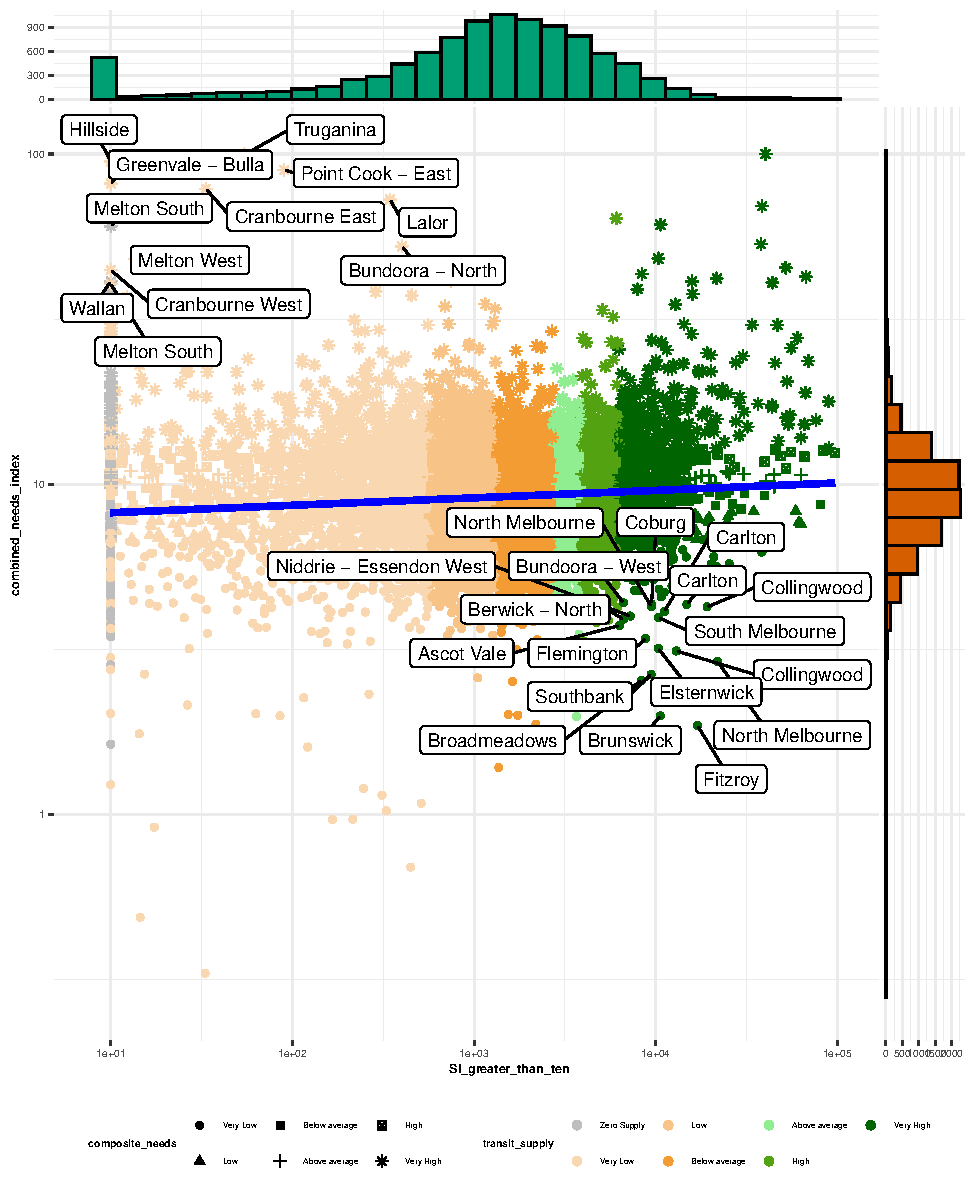
\includegraphics{ReynoldsCurrieQu2024_files/figure-latex/Greater_Melbourne_2016_needs_gap_scatterplot_figure-1.pdf}
\caption{Greater Melbourne 2016, SI and Combined Needs Index scores,
with SI scores \textless{} 10 rounded up to equal 10.}
\end{figure}

```

\begin{table}

\caption{\label{tab:Greater_Melbourne_2016_needs_gap_SA4_service_change}Greater Melbourne: SA1s with Very High needs but Very Low or Zero supply in 2016, by SA4 and change in SI by 2021}
\centering
\fontsize{8}{10}\selectfont
\begin{tabular}[t]{>{\raggedright\arraybackslash}p{2.5cm}|>{\raggedleft\arraybackslash}p{1cm}|>{\raggedleft\arraybackslash}p{1cm}|>{\raggedleft\arraybackslash}p{1cm}|>{\raggedleft\arraybackslash}p{1cm}|>{\raggedleft\arraybackslash}p{1cm}|>{\raggedleft\arraybackslash}p{1cm}|>{\raggedleft\arraybackslash}p{1cm}|>{\raggedleft\arraybackslash}p{1cm}|>{\raggedleft\arraybackslash}p{1cm}|>{\raggedleft\arraybackslash}p{1cm}}
\hline
Change & Inner & Inner South & Inner East & North East & North West & Outer East & South East & West & M'ton Pen. & Total\\
\hline
New or 30\%+ & 1.6\%  (6) & 6.6\% (24) & 14.5\%  (53) & 0.0\%  (0) & 5.5\% (20) & 3.0\% (11) & 0.5\% (2) & 0.0\% (0) & 0.0\% (0) & 31.8\% (116)\\
\hline
Increased 1 to 30\% & 2.5\%  (9) & 8.2\% (30) & 6.8\%  (25) & 2.5\%  (9) & 3.3\% (12) & 2.7\% (10) & 0.3\% (1) & 0.0\% (0) & 0.3\% (1) & 26.6\%  (97)\\
\hline
Within 1\% & 5.2\% (19) & 4.7\% (17) & 6.0\%  (22) & 6.3\% (23) & 0.3\%  (1) & 1.6\%  (6) & 0.5\% (2) & 0.0\% (0) & 0.3\% (1) & 24.9\%  (91)\\
\hline
Reduced, withdrawn, never & 2.7\% (10) & 3.6\% (13) & 2.5\%   (9) & 1.6\%  (6) & 0.8\%  (3) & 4.4\% (16) & 1.1\% (4) & 0.0\% (0) & 0.0\% (0) & 16.7\%  (61)\\
\hline
Total & 12.1\% (44) & 23.0\% (84) & 29.9\% (109) & 10.4\% (38) & 9.9\% (36) & 11.8\% (43) & 2.5\% (9) & 0.0\% (0) & 0.5\% (2) & 100.0\% (365)\\
\hline
\end{tabular}
\end{table}

\bibliography{References.bib, packages.bib}


\end{document}
